\newpage{\ }
\cleardoublepage

\chapter{Apéndice Capítulo 2}\label{append_02}

\section{Condiciones atmosféricas en el período de estudio}

\begin{figure}[H]
    \centering
    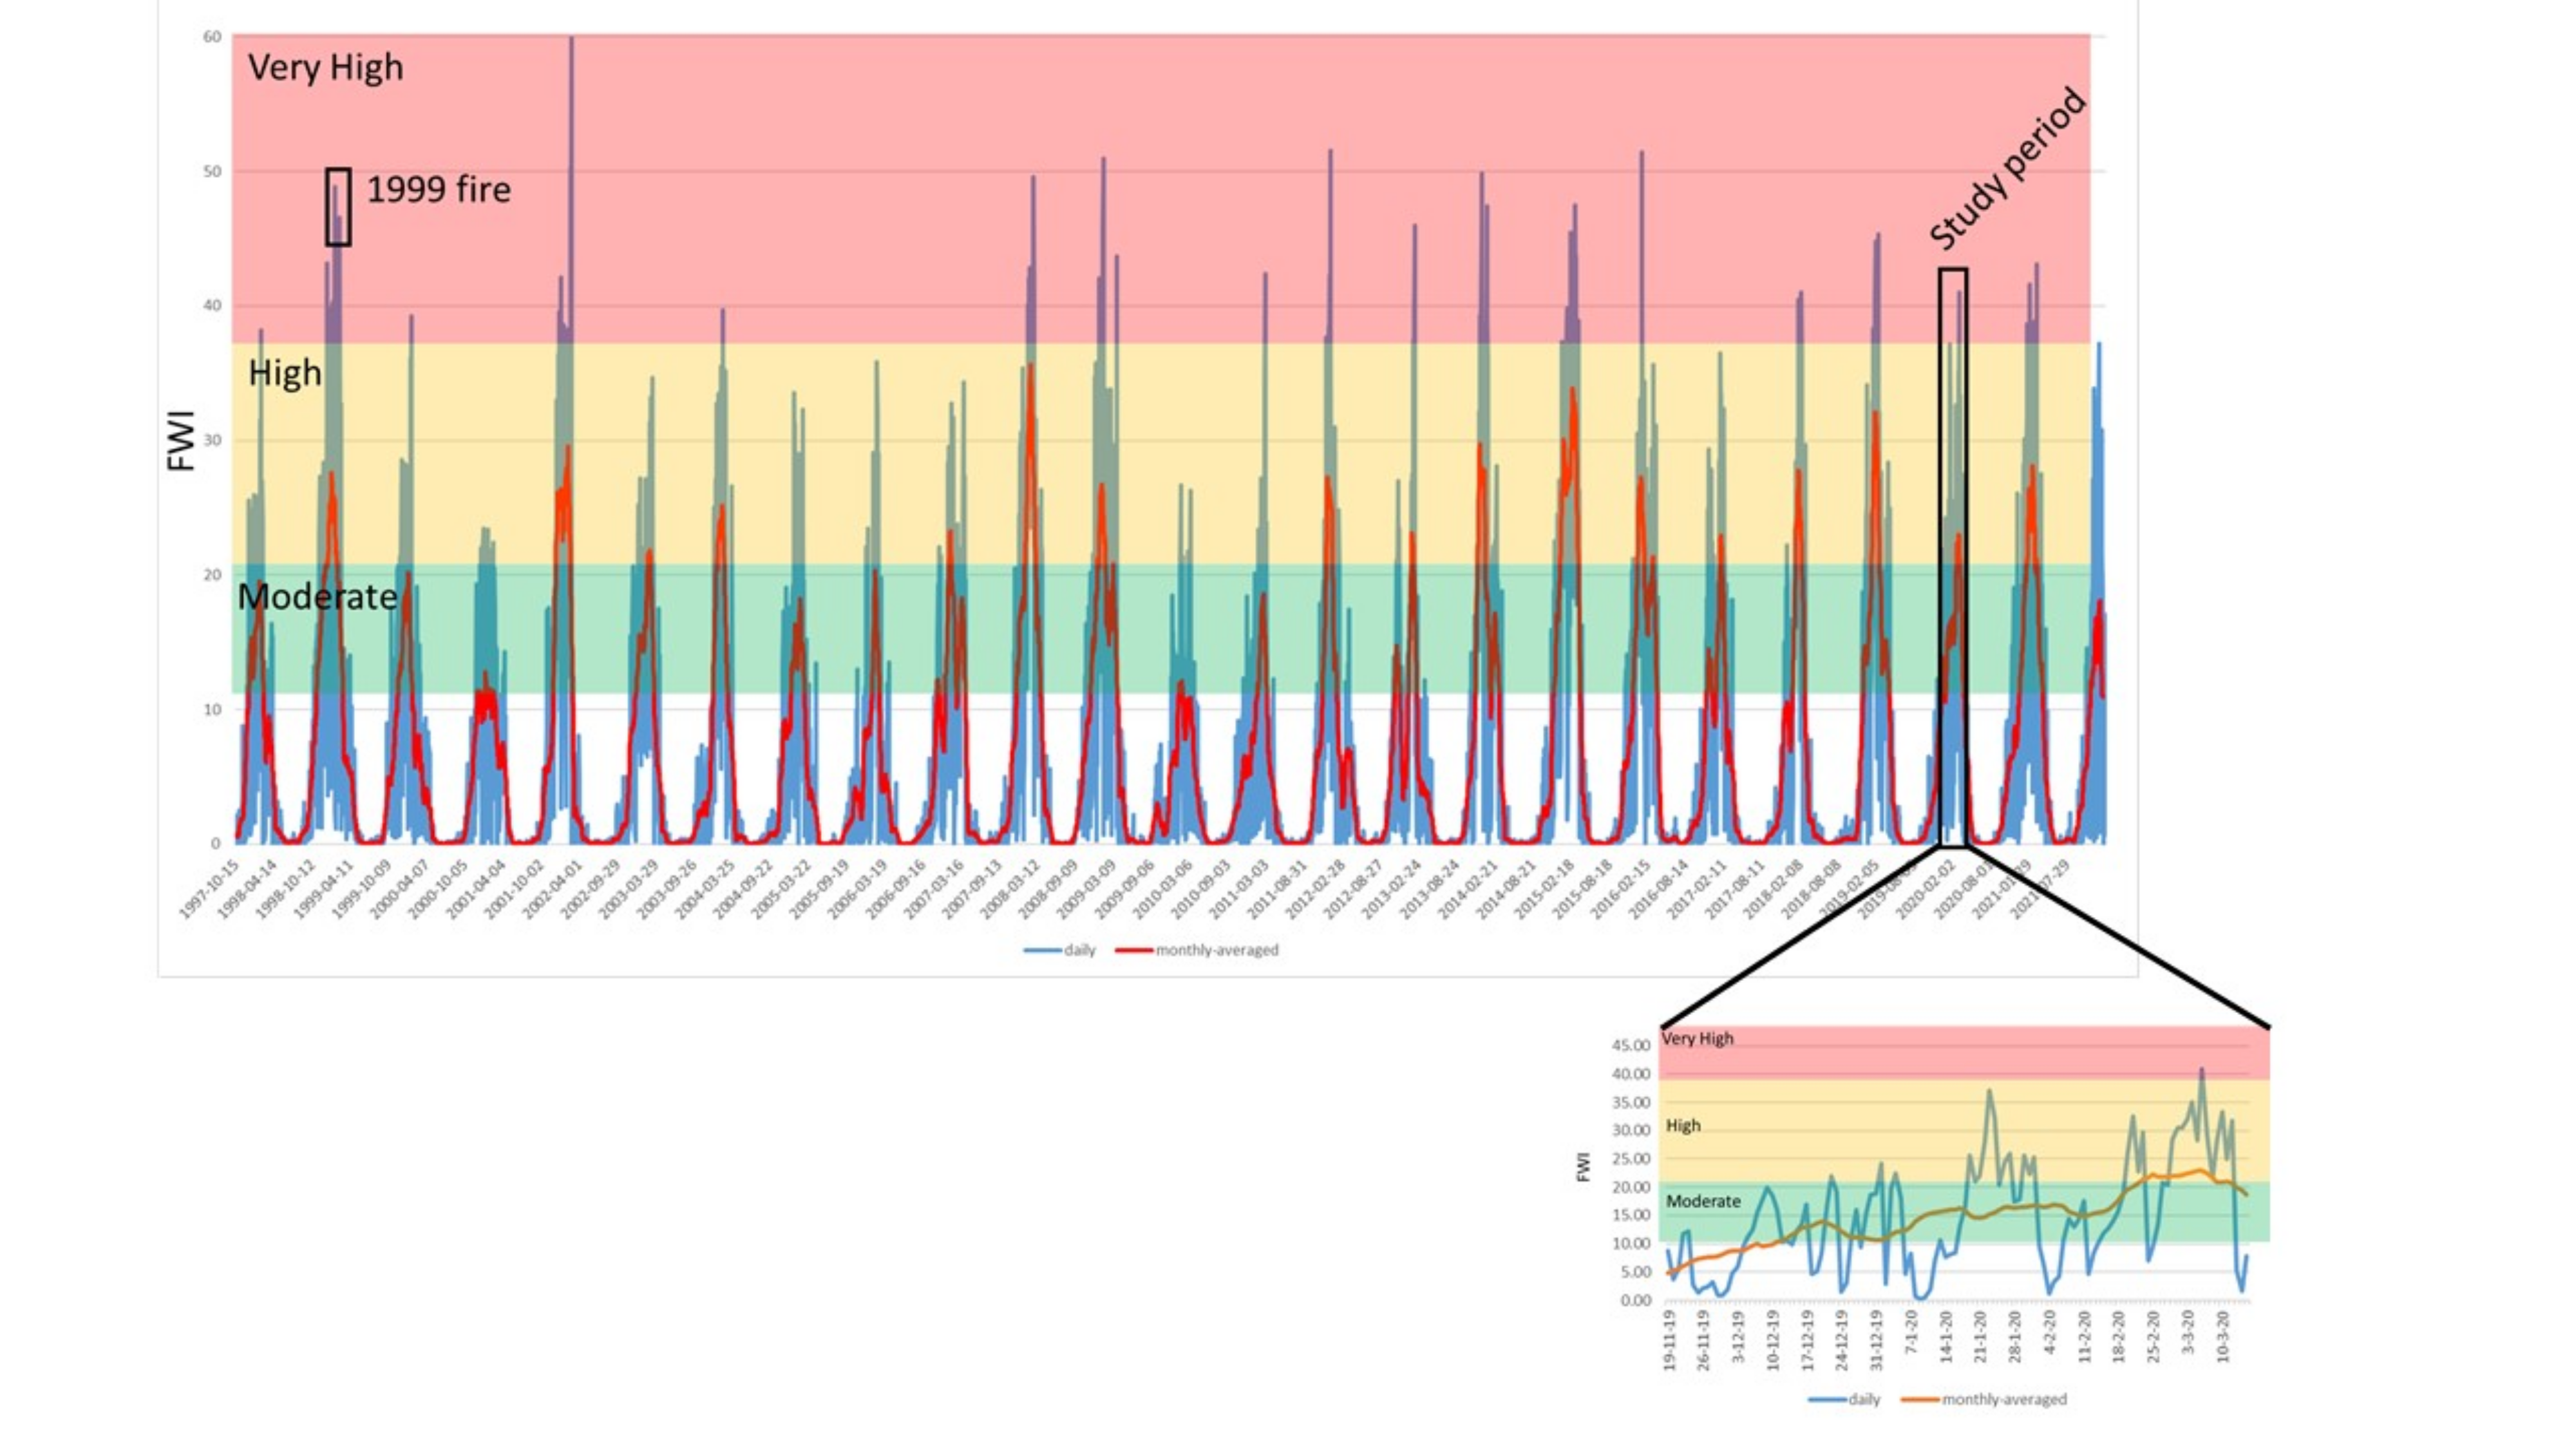
\includegraphics[width=16cm]{figuras/cap2/S01) fwi ts.png}
    \caption[FWI en el período de estudio.]{Fire Weather Index (FWI) diario (línea azul) y promedio mensual (línea roja) calculado a largo plazo (1998-2022) (arriba, izquierda) y entre el 19 de noviembre de 2019 y el 15 de marzo de 2020 (abajo, derecha) basados en el reanálisis de ERA5 del ECMWF (European Centre for Medium-Range Weather Forecasts/Copernicus Emergency Management Service; \citealt{vitolo_era5-based_2020}). Los colores de fondo indican las clases de peligro de incendio según el Sistema Europeo de Información sobre Incendios Forestales (EFFIS; \citealt{san-miguel-ayanz_comprehensive_2012}): moderado (11.2 a 21.3; verde), alto (21.3 a 38; amarillo) y muy alto (38 a 50; rojo). Los rectángulos negros señalan los valores del FWI durante el incendio de 1999 (rectángulo izquierdo) y durante el período de estudio (rectángulo derecho).}
    \label{fig:cap2-S01}
\end{figure}

\FloatBarrier

\section{Estructura de la vegetación}\label{append:veg-structure}

Evaluamos la composición de especies para explorar sus efectos sobre el contenido de humedad del combustible y caracterizamos la estructura del combustible para evaluar si nuestros sitios mostraban los mismos patrones descritos por \citet{paritsis_positive_2015} y \citet{tiribelli_changes_2018}, quienes analizaron tamaños de muestra y áreas de estudio más grandes. Construimos perfiles verticales de combustible utilizando el método de intersección con varilla \citet{paritsis_positive_2015, tiribelli_changes_2018}. En 30-60 puntos ubicados en cuadrículas rectangulares (con al menos 2 m entre puntos) en cada sitio, colocamos una varilla de 4 m de altura dividida en 16 segmentos de 25 cm y registramos la presencia de combustible fino (hojas o ramas finas $< 6$ mm) en un radio de 10 cm alrededor de la varilla en cada segmento, identificando las especies leñosas y si se trataba de material vivo o muerto. También medimos la profundidad de la capa de hojarasca, estimamos visualmente su cobertura (proporción) en cuadrantes de 1 m$^2$ en cada punto donde se colocó la varilla, y estimamos la cobertura del dosel a 1.5 m de altura en 30 puntos por sitio utilizando un \textit{smartphone} y la aplicación HabitApp. En general, los patrones de estructura de la vegetación coincidieron con los reportados por \citet{paritsis_positive_2015} y \citet{tiribelli_changes_2018}, aunque los sitios de matorral cerrado podrían tener una menor cantidad de combustible que el promedio estimado por \citet{tiribelli_changes_2018}.

Los combustibles finos estaban compuestos principalmente por combustible vivo (hojas y ramas finas de $< 6$ mm de diámetro), y la proporción de combustible vivo (número de segmentos con combustible sobre el número total de segmentos) fue más alta en los bosques jóvenes, seguida por los bosques maduros o los matorrales cerrados, alcanzando su mínimo en los matorrales abiertos. Considerando solo los combustibles muertos, no se observó un patrón claro de variación entre comunidades. Sin distinguir entre combustibles vivos y muertos, encontramos el mismo patrón que en los combustibles vivos, dado que estos eran los más abundantes (Fig.~\ref{fig:cap2-S02}).

\begin{figure}
    \centering
    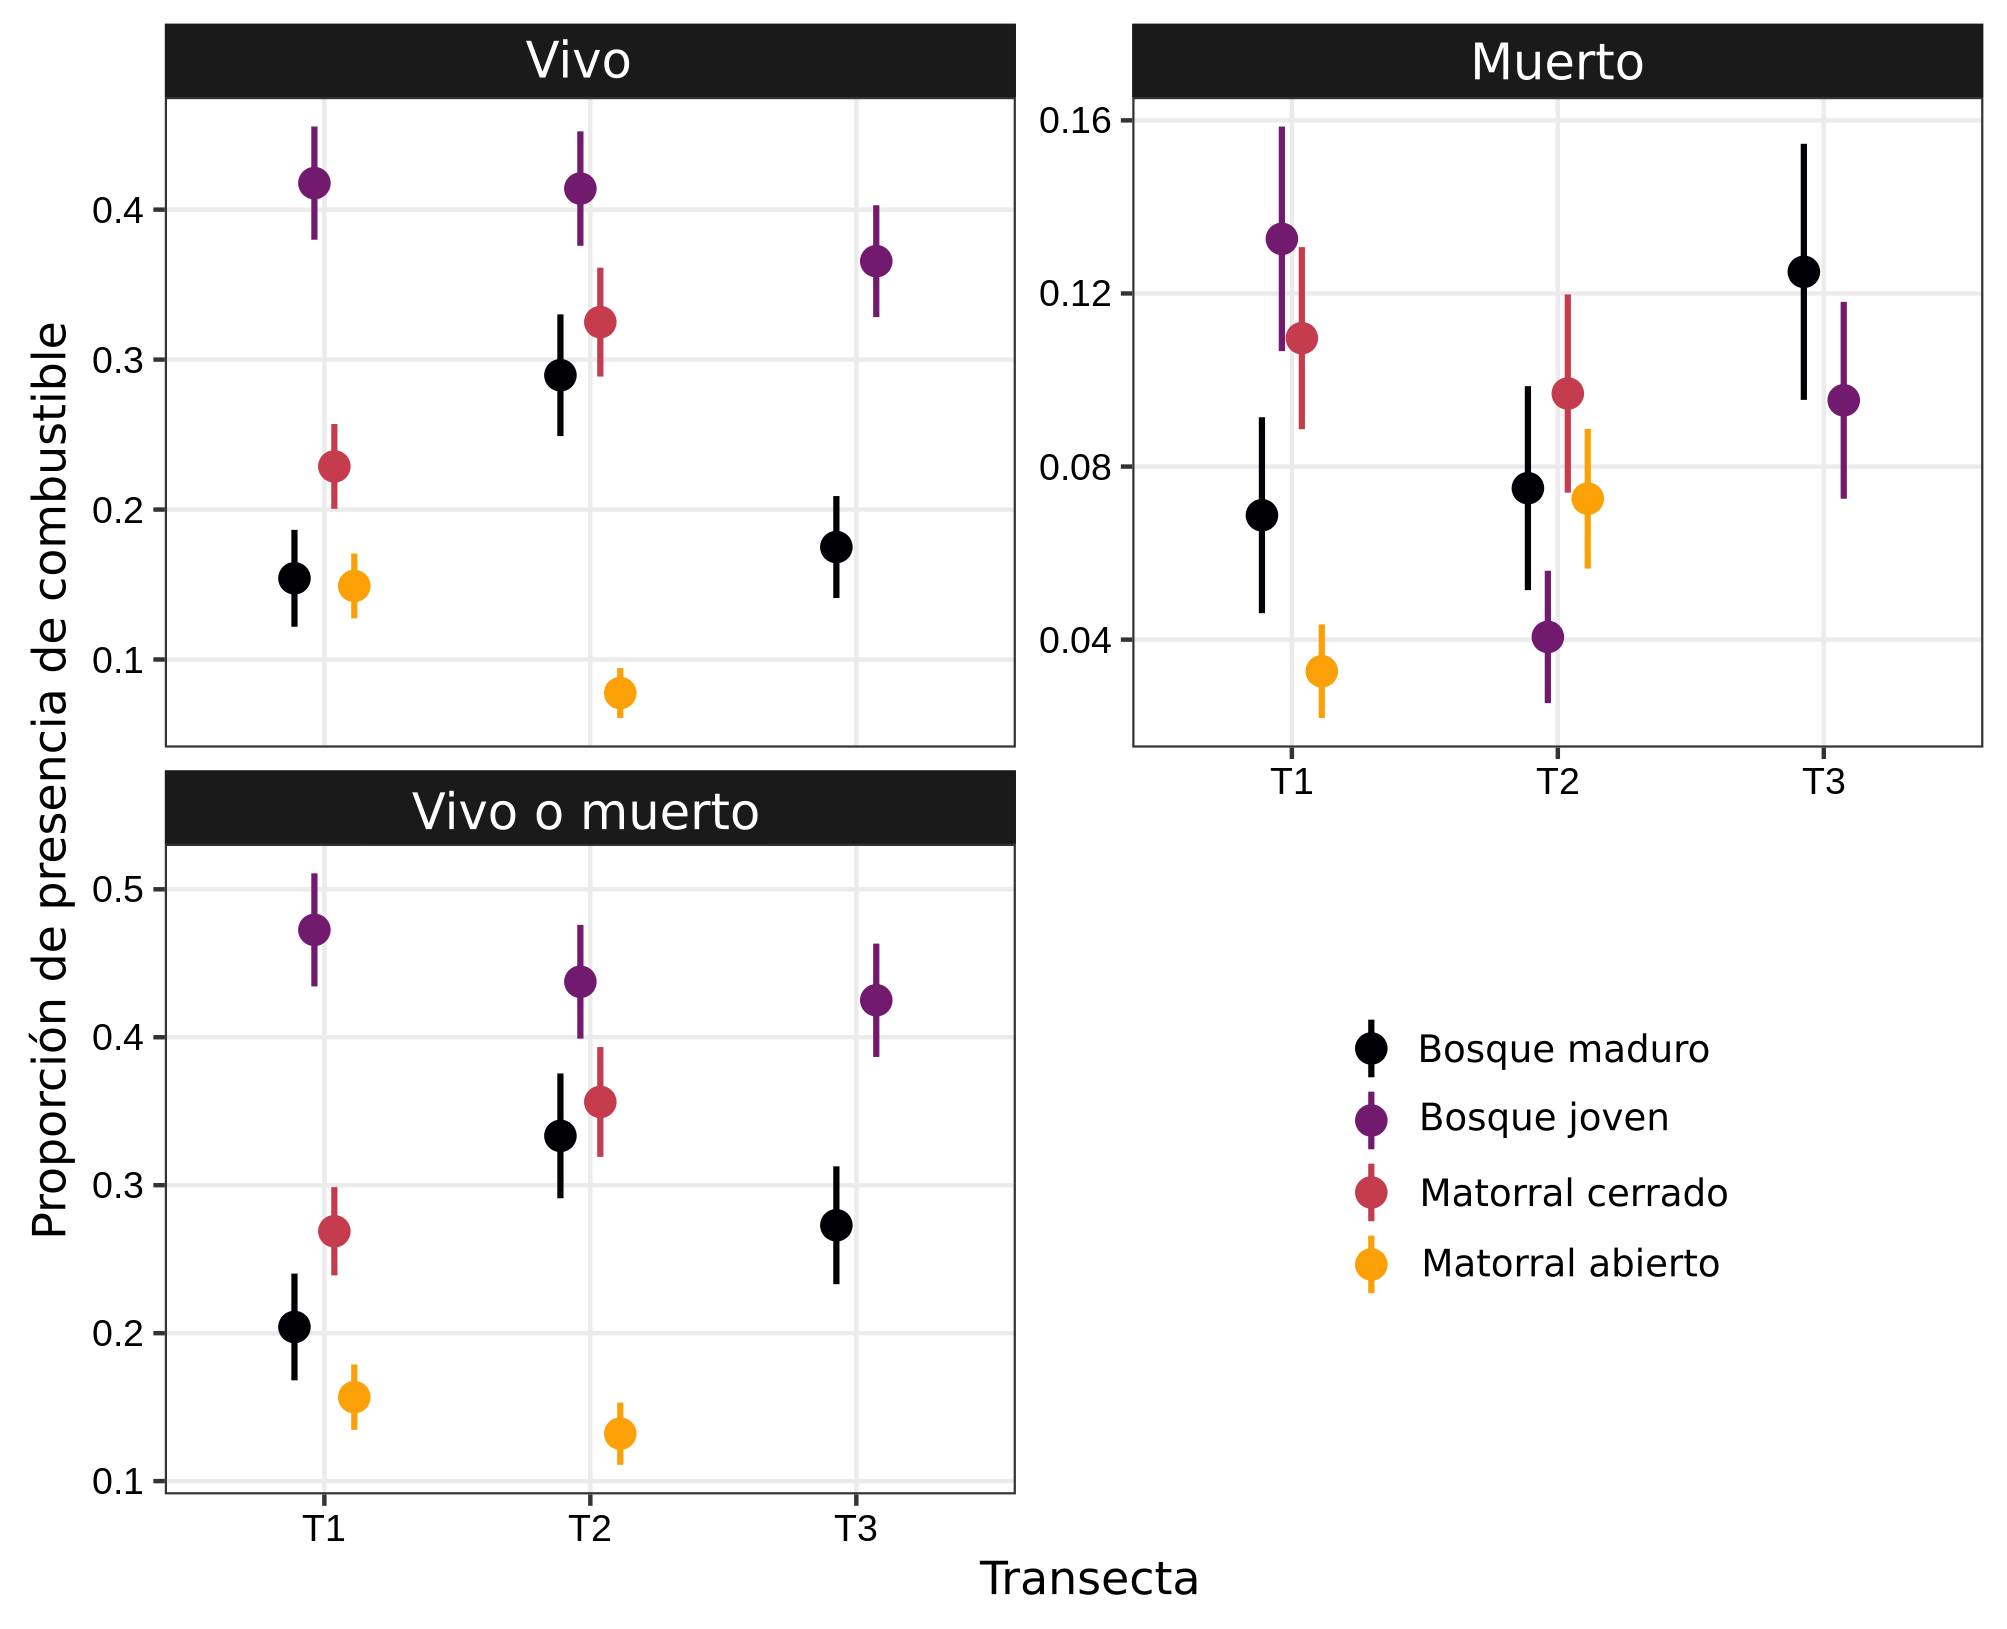
\includegraphics[width=16cm]{figuras/cap2/S02) prop fine fuel.png}
    \caption[Proporción de presencia de combustible por comunidad y transecta.]{Proporción de presencia de combustible por comunidad y transecta. Los puntos muestran la proporción de segmentos de la varilla con presencia de combustible, sin distinguir altura ni punto de muestreo. Dado que cada punto tenía 16 segmentos (varilla de 4 m, 25 cm por segmento), un sitio con 30 puntos tendría 30 $\times$ 16 = 480 segmentos. Las barras muestran $\pm 2$ desvíos estándar para las proporciones, calculadas según \citet[página 17]{GelmanHill2006}.}
    \label{fig:cap2-S02}
\end{figure}

Para analizar la continuidad vertical del combustible, ajustamos un Modelo Aditivo Generalizado (GAM) Binomial en el que la probabilidad de presencia de combustible varió como una función no lineal suave de la altura, la cual varió entre tipos de combustible (vivo, muerto y vivo o muerto), transectas y comunidades. Utilizamos splines cúbicas con 11 funciones base y ajustamos el modelo con el paquete de R \texttt{mgcv} \citep{wood_generalized_2017}. Los perfiles verticales de combustible muestran que los bosques jóvenes presentan la mayor probabilidad de presencia de combustible en todas las alturas, seguidos por los bosques maduros o los matorrales cerrados. Los matorrales abiertos muestran la menor probabilidad de presencia de combustible, excepto a baja altura, donde es alta debido a la presencia de la capa de pastos. Los matorrales cerrados presentan una menor probabilidad de presencia de combustible a mayor altura (4 m) porque la altura de los arbustos/árboles alcanza aproximadamente los 3 m, pero la continuidad del combustible es alta hasta esa altura (Fig.~\ref{fig:cap2-S03}).

\begin{figure}
    \centering
    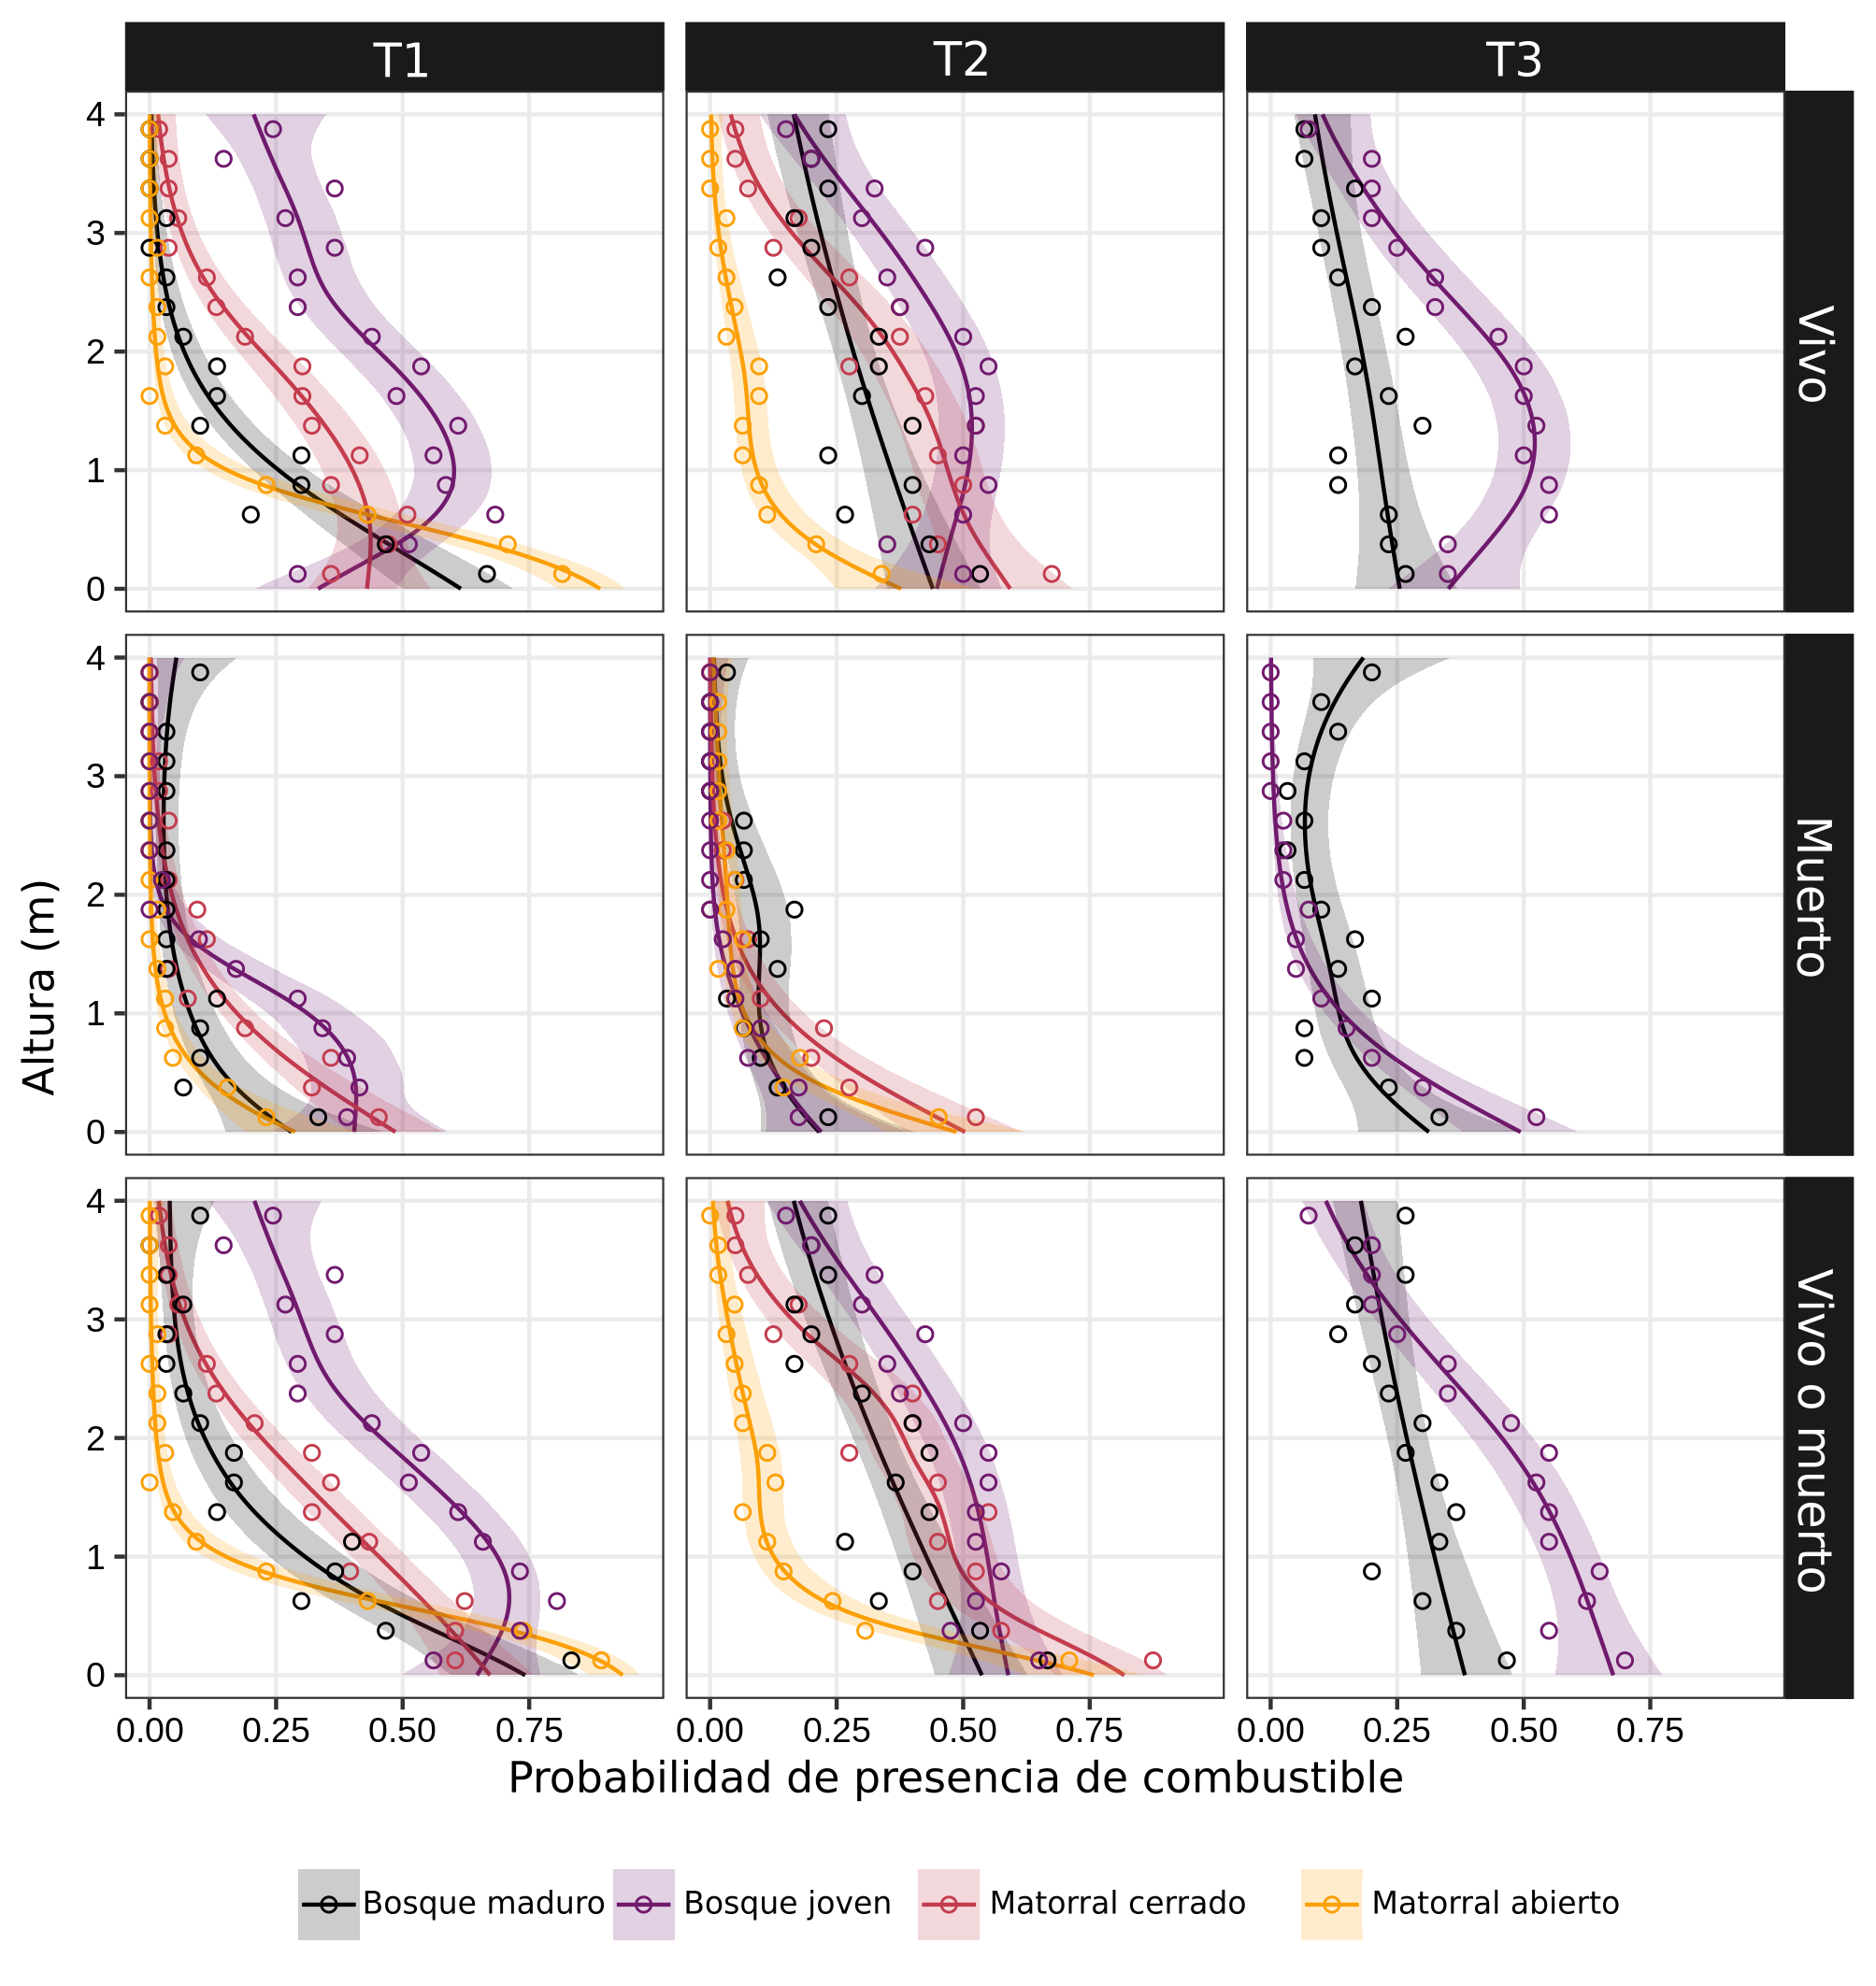
\includegraphics[width=16cm]{figuras/cap2/S03) fine fuel profile.png}
    \caption[Perfil vertical de combustible.]{Probabilidad de presencia de combustible (líneas) o proporción observada (puntos) en función de la altura, transecta y comunidad. Las líneas muestran la predicción del GAM ajustado, y las bandas sombreadas representan los intervalos de confianza del 95 \%. La variable predictora (altura) se muestra en el eje y para destacar que estos son perfiles verticales de combustible. Dado nuestro método de muestreo, la probabilidad de presencia de combustible se interpreta como la probabilidad de encontrar combustible fino en un segmento de 25 cm de altura centrado en un valor específico de altura.}
    \label{fig:cap2-S03}
\end{figure}

\citet{paritsis_positive_2015} estudiaron bosques alpinos de \textit{Nothofagus pumilio} y matorrales cercanos, mientras que \citet{tiribelli_changes_2018} estudiaron bosques de \textit{Nothofagus dombeyi} y matorrales, como hicimos nosotros. Ambos estudios encontraron patrones similares en general. \citet{tiribelli_changes_2018} estimaron una mayor proporción de combustible fino en los matorrales cerrados que en los bosques jóvenes 20 años después del incendio, por lo que la diferencia opuesta que encontramos probablemente no sea un patrón general. Además, el matorral cerrado en la transecta 1 tuvo una proporción de combustible baja en comparación con las predicciones de \citet{tiribelli_changes_2018}.
Cabe destacar que, dado que consideramos un radio de 10 cm para definir la presencia de combustible con el método de intersección con varilla, es razonable encontrar valores ligeramente más altos que los reportados por \citet{tiribelli_changes_2018}.

La profundidad de la hojarasca en los bosques maduros tendió a ser menor que en los bosques jóvenes y los matorrales cerrados, pero similar o mayor que en los matorrales abiertos. La cobertura de hojarasca fue más baja en los matorrales abiertos, mientras que las diferencias entre las demás comunidades fueron pequeñas y variables entre transectas (Fig.~\ref{fig:cap2-S04}).

\begin{figure}
    \centering
    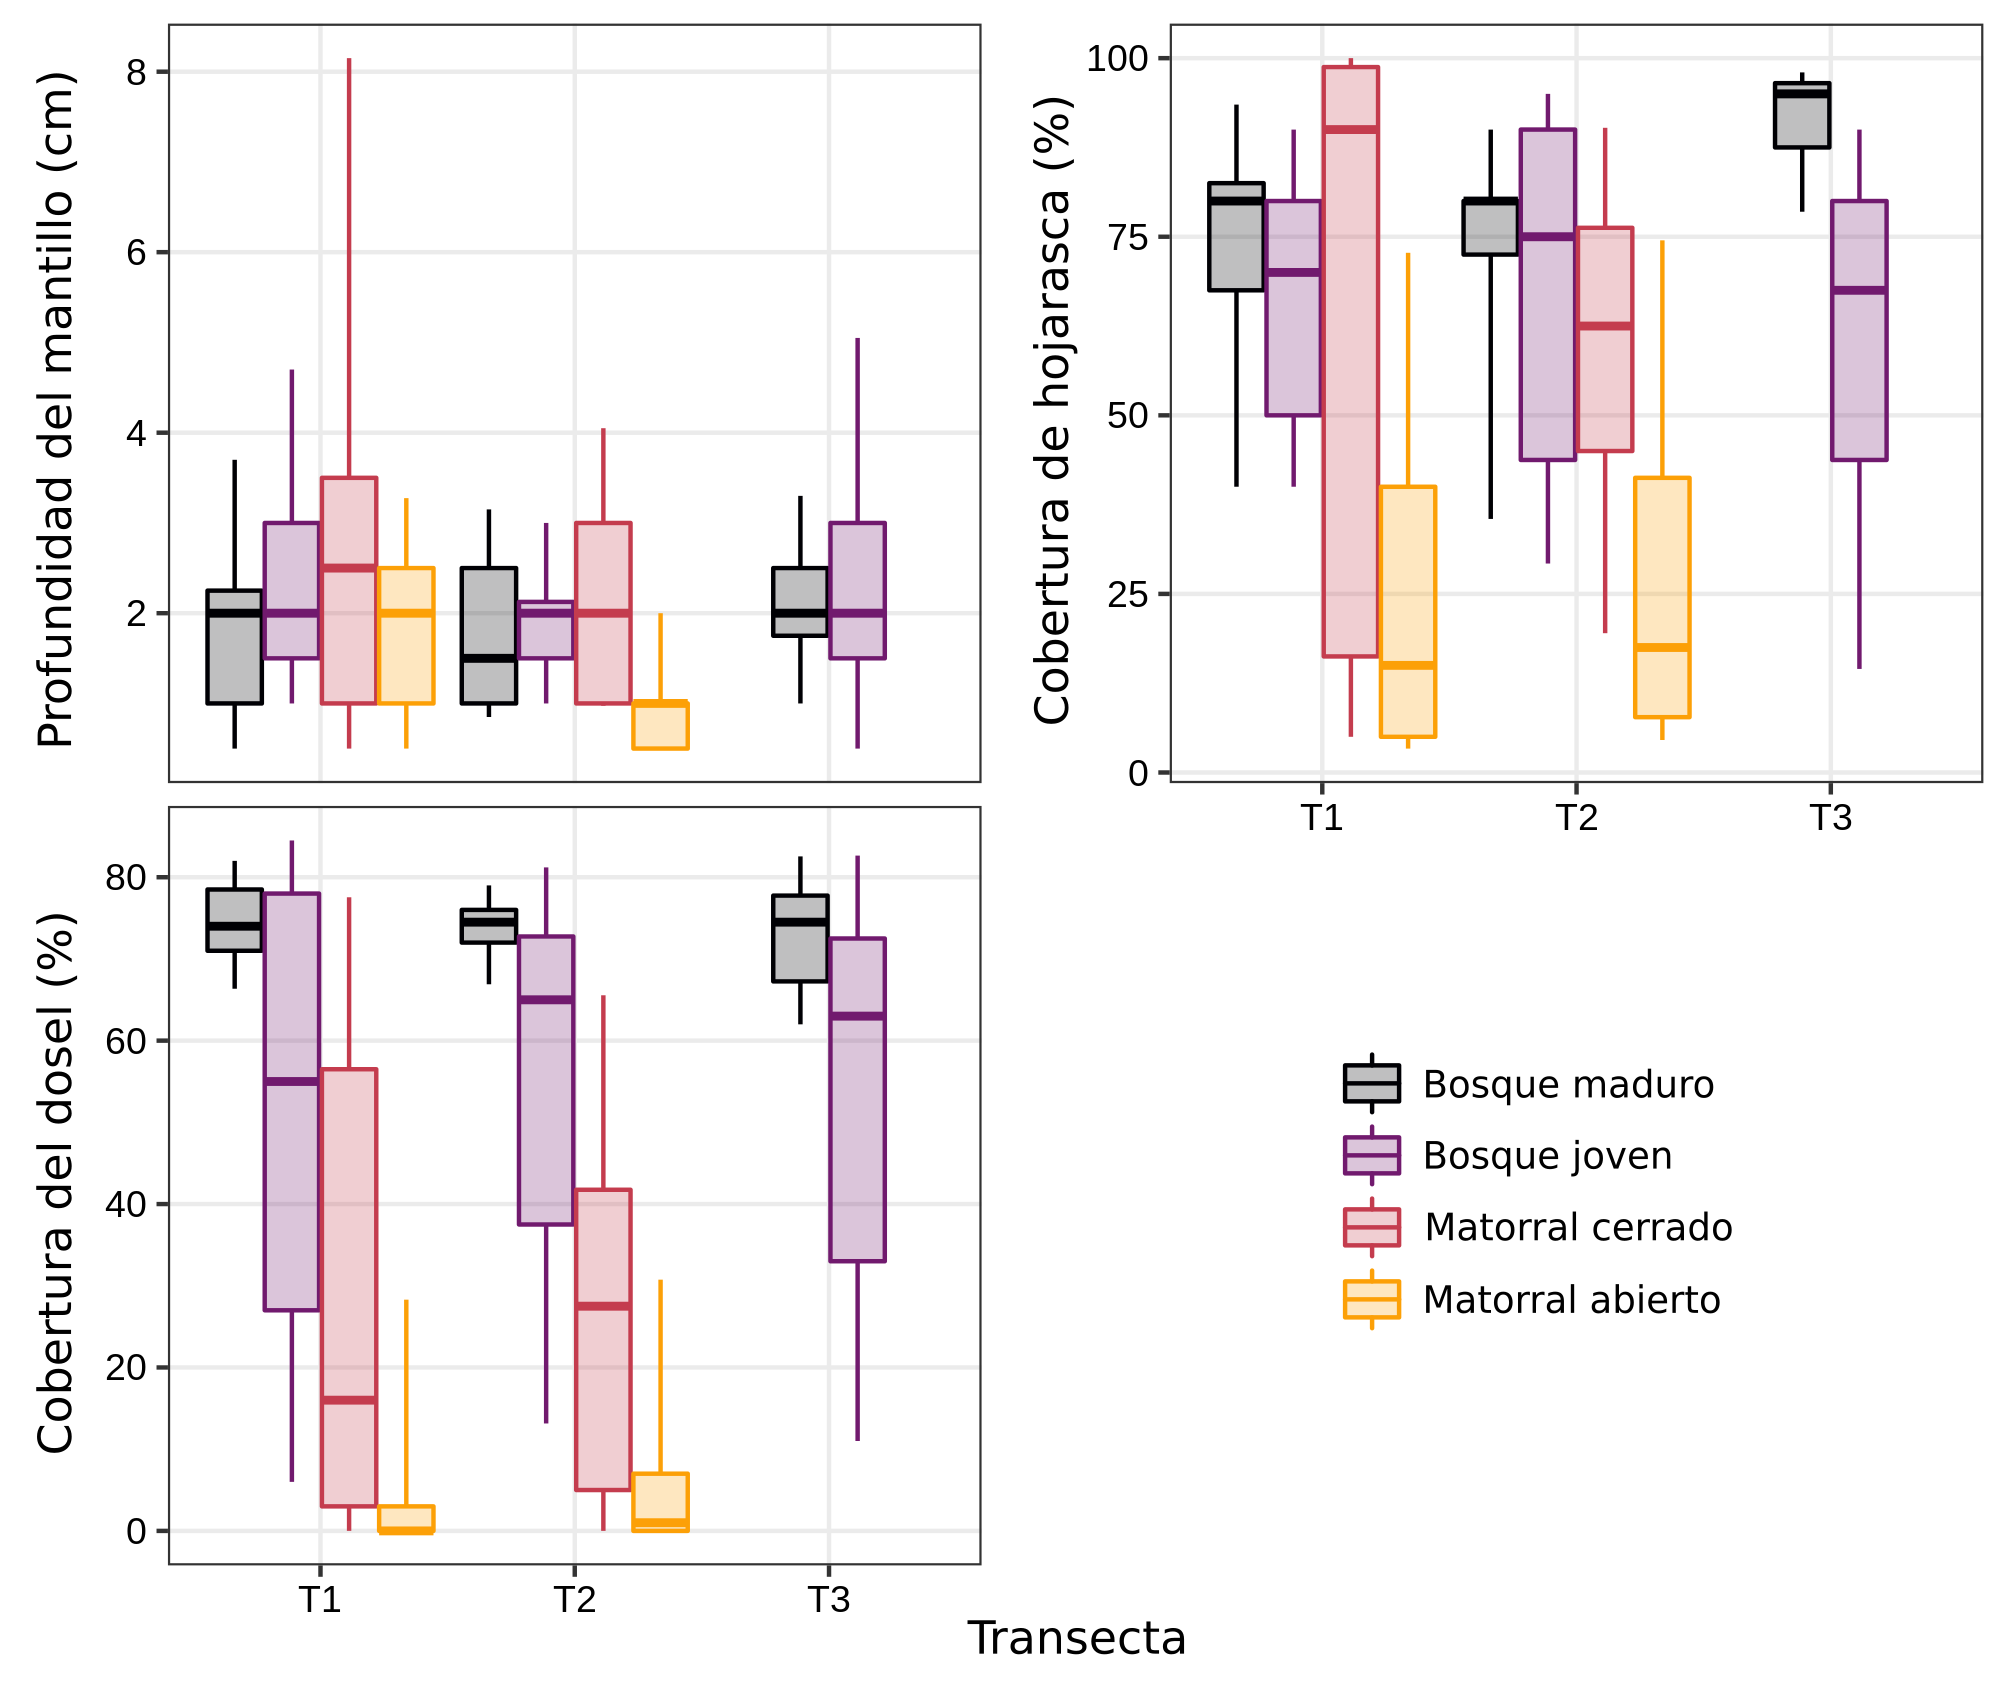
\includegraphics[width=16cm]{figuras/cap2/S04) fuel structure others.png}
    \caption[Profundidad y cobertura del mantillo y cobertura del dosel.]{Diagramas de caja para la profundidad de la hojarasca, la cobertura de la hojarasca y la cobertura del dosel por encima de 1.5 m de altura, agrupados por comunidad y transecta (percentiles 5 \%, 25 \%, 50 \%, 75 \% y 95 \%).}
    \label{fig:cap2-S04}
\end{figure}

La cobertura del dosel mostró una notable variación entre comunidades. Fue más alta en los bosques maduros y más baja en los matorrales abiertos, y estas comunidades mostraron poca variabilidad. Los bosques jóvenes y los matorrales cerrados mostraron valores intermedios, siendo más altos en los bosques jóvenes, y ambas comunidades mostraron alta variabilidad. Estos patrones fueron consistentes entre transectas (Fig.~\ref{fig:cap2-S04}).

\FloatBarrier

\section{Composición de especies}\label{append:sp-comp}

\begin{table}[ht]
\centering
\caption[Abundancia relativa de especies por comunidad y transecta.]{Abundancia relativa (\%) de especies por comunidad y transecta considerando únicamente el combustible vivo. Las especies están ordenadas de mayor a menor abundancia, considerando todos los sitios en conjunto. La abundancia relativa se derivó de los datos de intersección con varilla, describiendo la vegetación hasta 4 m de altura.}
\resizebox{\textwidth}{!}{%
\begin{tabular}{l|cccc|cccc|cc}
\toprule
Transecta & \multicolumn{4}{c}{T1} & \multicolumn{4}{c}{T2} & \multicolumn{2}{c}{T3} \\
Especie/Comunidad & BM & BJ & MC & MA & BM & BJ & MC & MA & BM & BJ \\
\hline
\textit{Nothofagus dombeyi} &  12.7 & 45.4 & 0 & 0 & 36.4 & 79.1 & 19.2 & 15.4 & 9.3 & 70.4 \\
Herbáceas &  12.7 & 5.4 & 8 & 62.6 & 6 & 3.9 & 12.9 & 29.5 & 1.2 & 7.4 \\
\textit{Schinus patagonicus} &  29.1 & 8.6 & 2.2 & 3.7 & 21.2 & 3.9 & 18.8 & 26.9 & 16.3 & 3.7 \\
\textit{Chusquea culeou} &  25.3 & 3.2 & 0 & 0 & 23.2 & 0.4 & 0 & 0 & 60.5 & 14.4 \\
\textit{Mutisia spinosa} &  0 & 14.6 & 8.8 & 27.8 & 0 & 4.6 & 7.1 & 0 & 0 & 0 \\
\textit{Lomatia hirsuta} &  0 & 14.3 & 16.8 & 0 & 0 & 0 & 21 & 0 & 8.1 & 0.8 \\
\textit{Fabiana imbricata} &  0 & 0 & 19.5 & 2.7 & 0 & 0 & 14.3 & 23.1 & 0 & 0 \\
\textit{Aristotelia chilensis} &  11.4 & 7 & 0 & 0 & 6.6 & 3.9 & 0 & 0 & 0 & 1.2 \\
\textit{Nothofagus antarctica} &  0 & 0 & 19 & 0 & 0 & 0 & 2.7 & 0 & 0 & 0 \\
\textit{Maytenus boaria} &  1.3 & 0 & 7.1 & 1.6 & 0 & 0 & 0 & 1.3 & 0 & 0.8 \\
\textit{Austrocedrus chilensis} &  7.6 & 0.6 & 0 & 0 & 0 & 0 & 0 & 0 & 0 & 0 \\
\textit{Berberis microphylla} &  0 & 0 & 2.7 & 0 & 0.7 & 1.4 & 0.9 & 0 & 1.2 & 0 \\
\textit{Diostea juncea} &  0 & 0 & 4.4 & 1.6 & 0 & 0 & 0 & 0 & 0 & 0 \\
\textit{Embothrium coccineum} &  0 & 0 & 2.2 & 0 & 3.3 & 0 & 0 & 0 & 0 & 0 \\
\textit{Discaria chacaye} &  0 & 0 & 4.4 & 0 & 0 & 0.4 & 0.4 & 0 & 0 & 0 \\
\textit{Baccharis sp.} &  0 & 0 & 3.5 & 0 & 0 & 0.4 & 0 & 0 & 0 & 0 \\
\textit{Ribes magellanicum} &  0 & 1 & 0 & 0 & 0 & 1.1 & 0.4 & 0 & 0 & 1.2 \\
\textit{Gaultheria mucronata} &  0 & 0 & 0 & 0 & 0 & 1.1 & 1.3 & 1.3 & 0 & 0 \\
\textit{Maytenus chubutensis} &  0 & 0 & 0 & 0 & 0 & 0 & 0.9 & 0 & 2.3 & 0 \\
\textit{Adesmia sp.} &  0 & 0 & 0 & 0 & 0 & 0 & 0 & 2.6 & 0 & 0 \\
\textit{Berberis serratodentata} &  0 & 0 & 0 & 0 & 2 & 0 & 0 & 0 & 0 & 0 \\
\textit{Myoschilos oblongum} &  0 & 0 & 1.3 & 0 & 0 & 0 & 0 & 0 & 0 & 0 \\
\textit{Maytenus magellanica} &  0 & 0 & 0 & 0 & 0 & 0 & 0 & 0 & 1.2 & 0 \\
\textit{Rosa rubiginosa} &  0 & 0 & 0 & 0 & 0.7 & 0 & 0 & 0 & 0 & 0 \\
\bottomrule
\end{tabular}%
}
\label{tab:sp-composition}
\end{table}


\begin{figure}
    \centering
    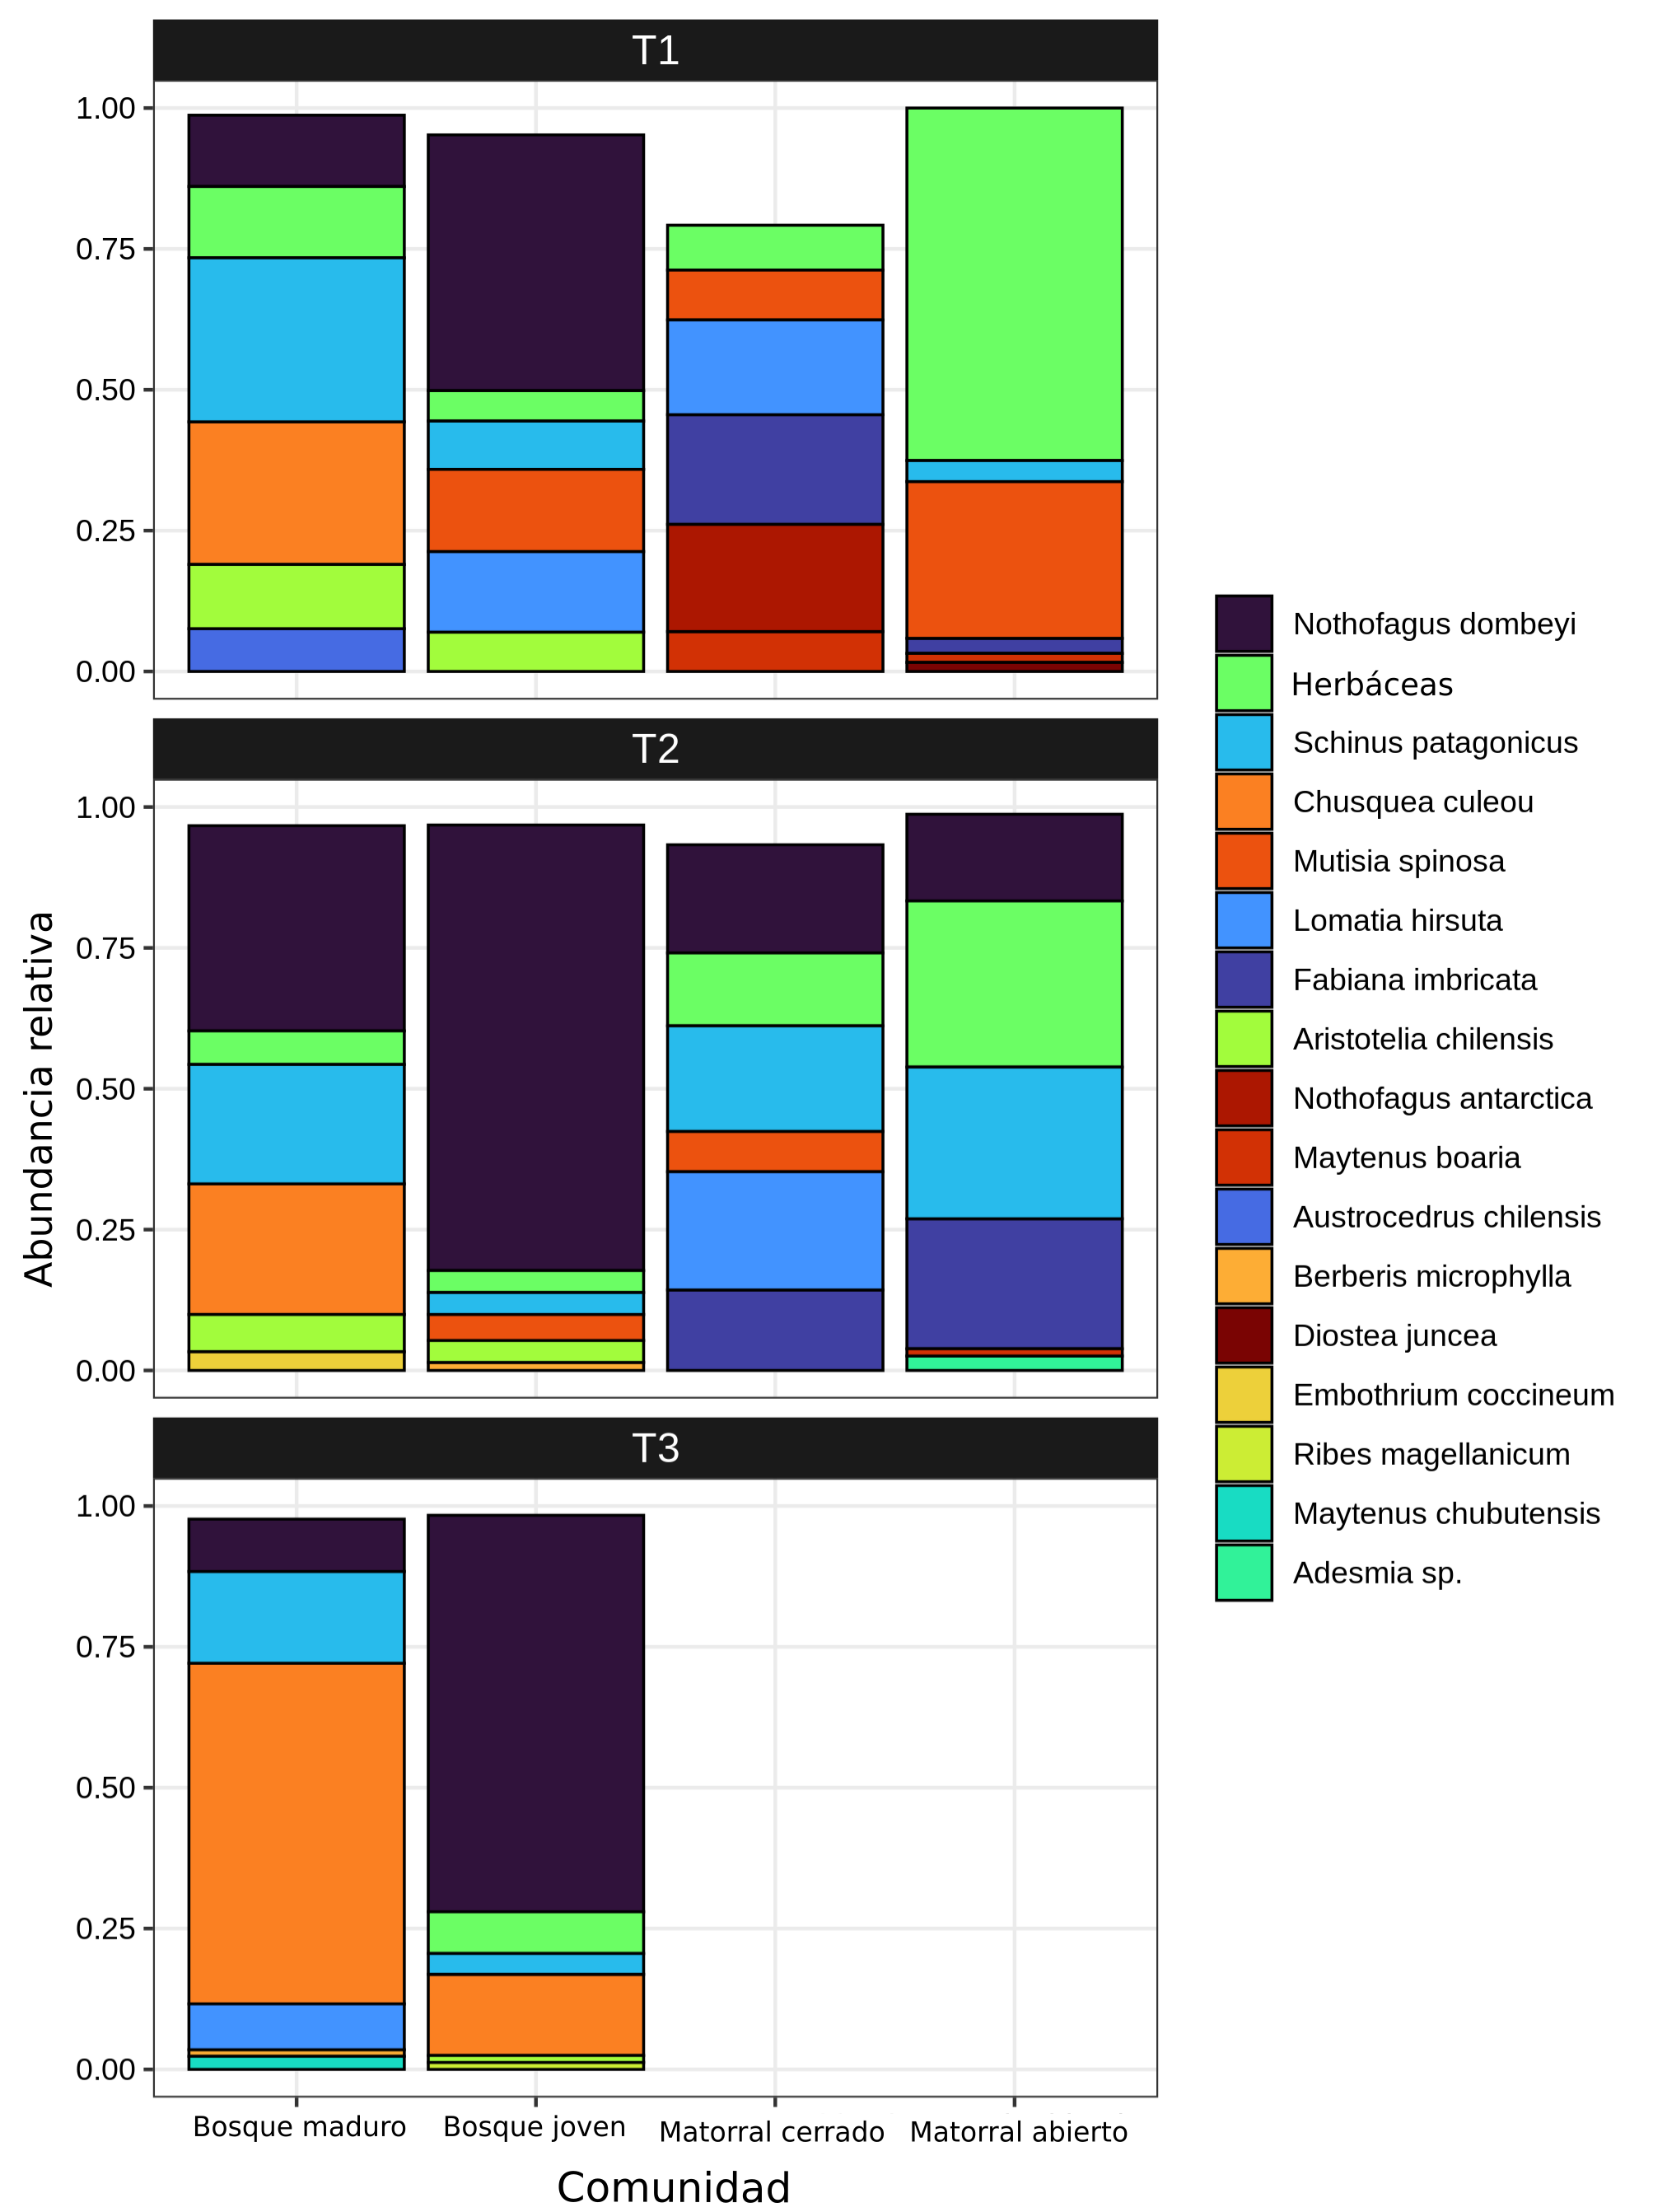
\includegraphics[width=16cm]{figuras/cap2/S05) composition.png}
    \caption[Composición de especies.]{Abundancia relativa de especies por comunidad y transecta para el combustible vivo. Solo se muestran las seis especies más abundantes en cada sitio para facilitar la visualización. La abundancia relativa se derivó de los datos de intersección con varilla, describiendo la vegetación hasta 4 m de altura.}
    \label{fig:cap2-S05}
\end{figure}

\FloatBarrier

\section{Figuras adicionales: datos y modelos de humedad del combustible}

\begin{figure}[H]
    \centering
    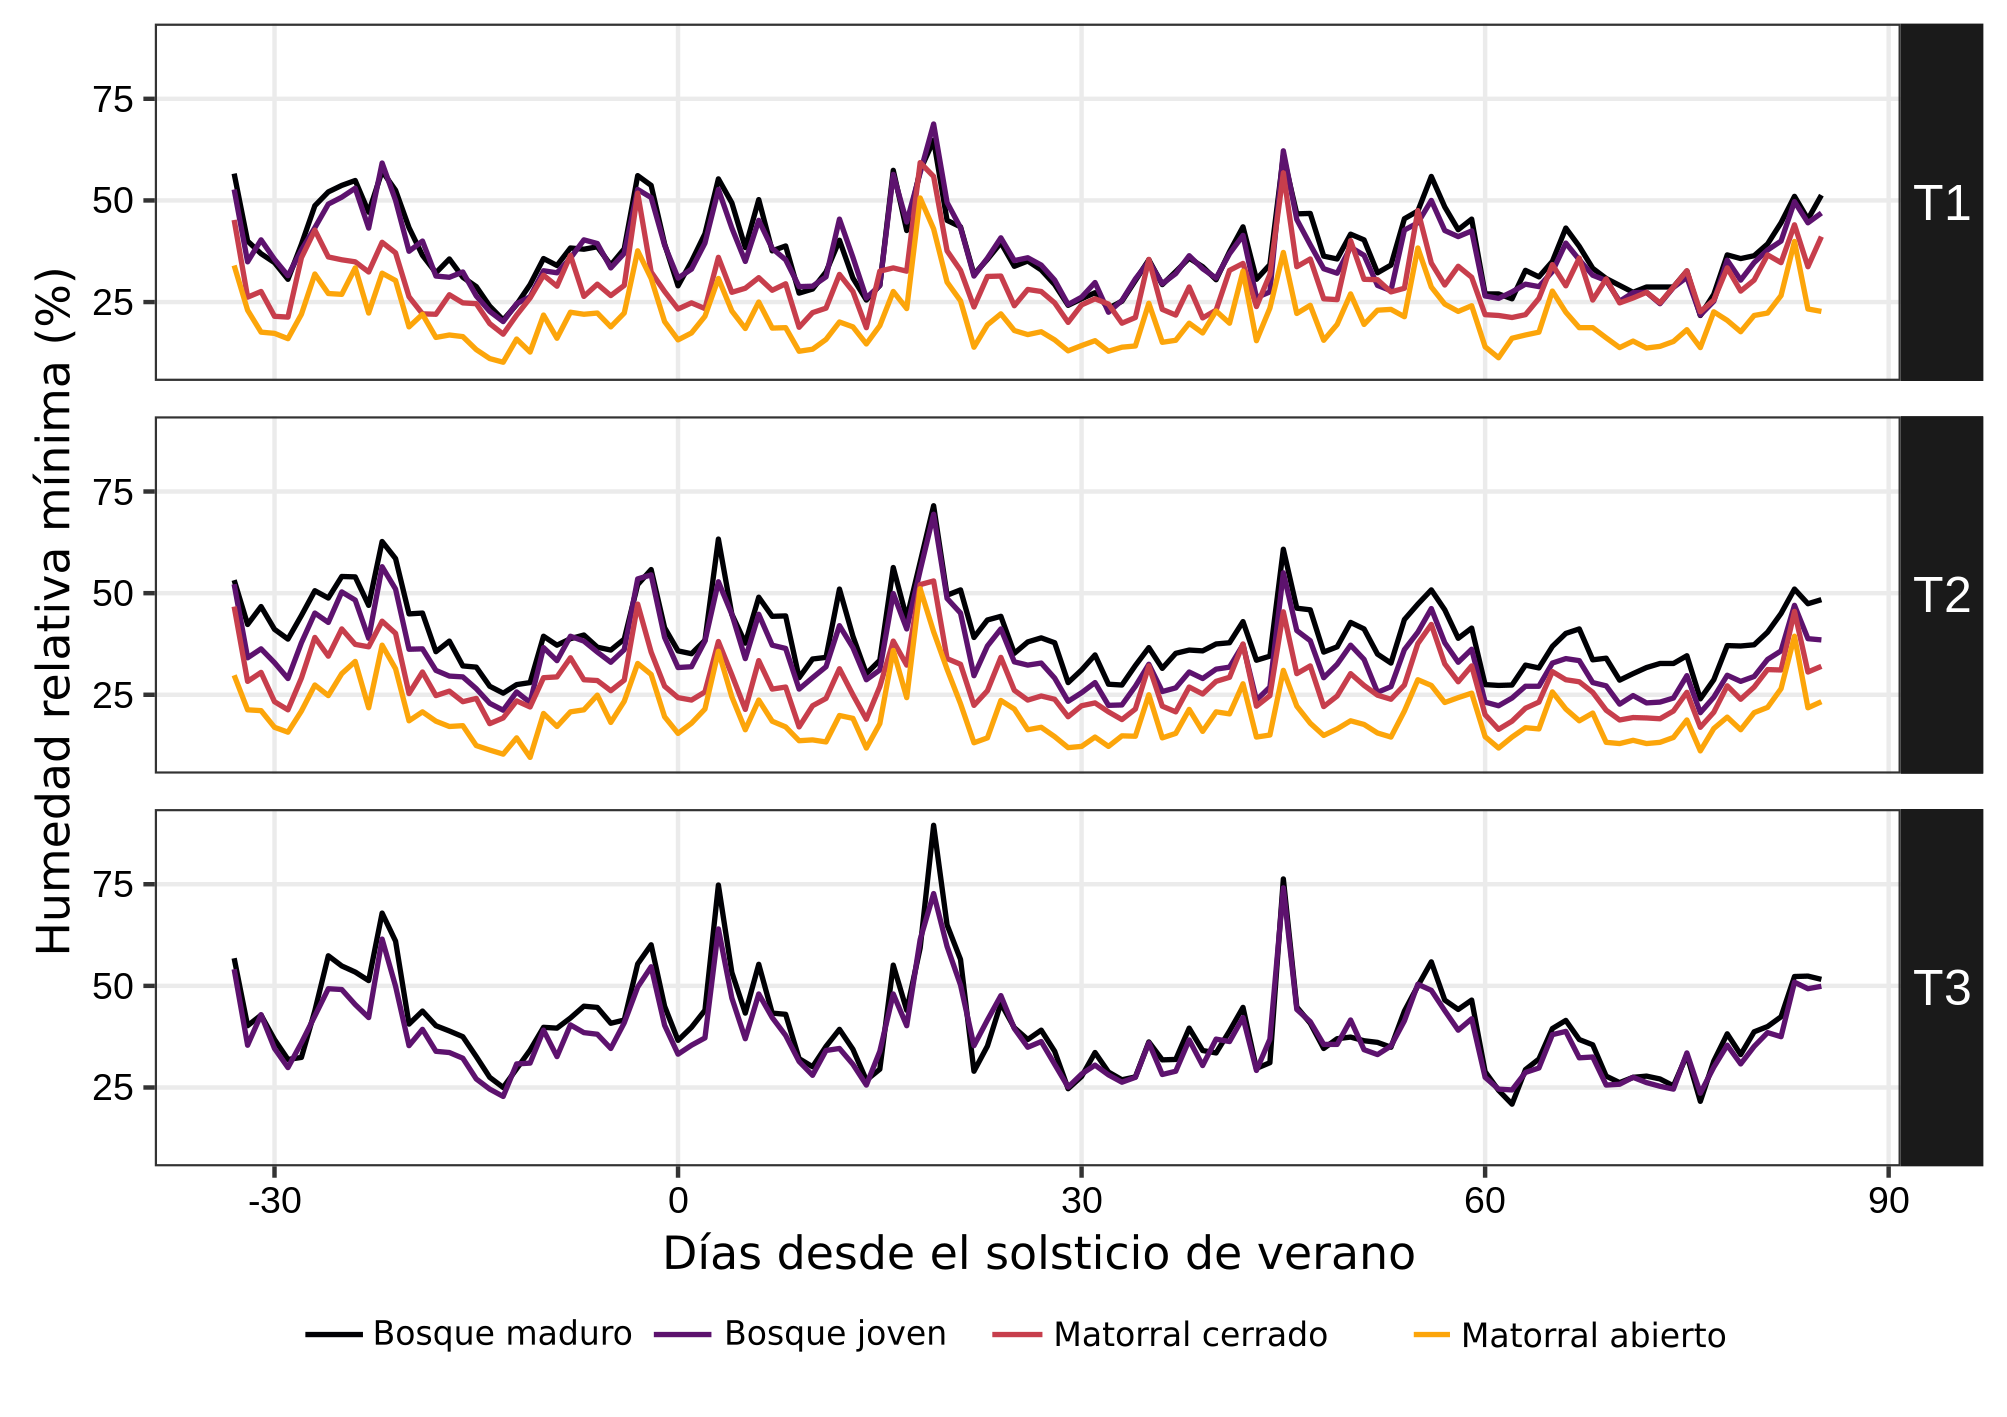
\includegraphics[width=16cm]{figuras/cap2/S06) air moisture ts.png}
    \caption[Humedad relativa del aire, series temporales.]{Humedad relativa mínima diaria (\%) a lo largo de la estación seca. El día cero corresponde al 21 de diciembre de 2019.}
    \label{fig:cap2-S06}
\end{figure}

\begin{figure}
    \centering
    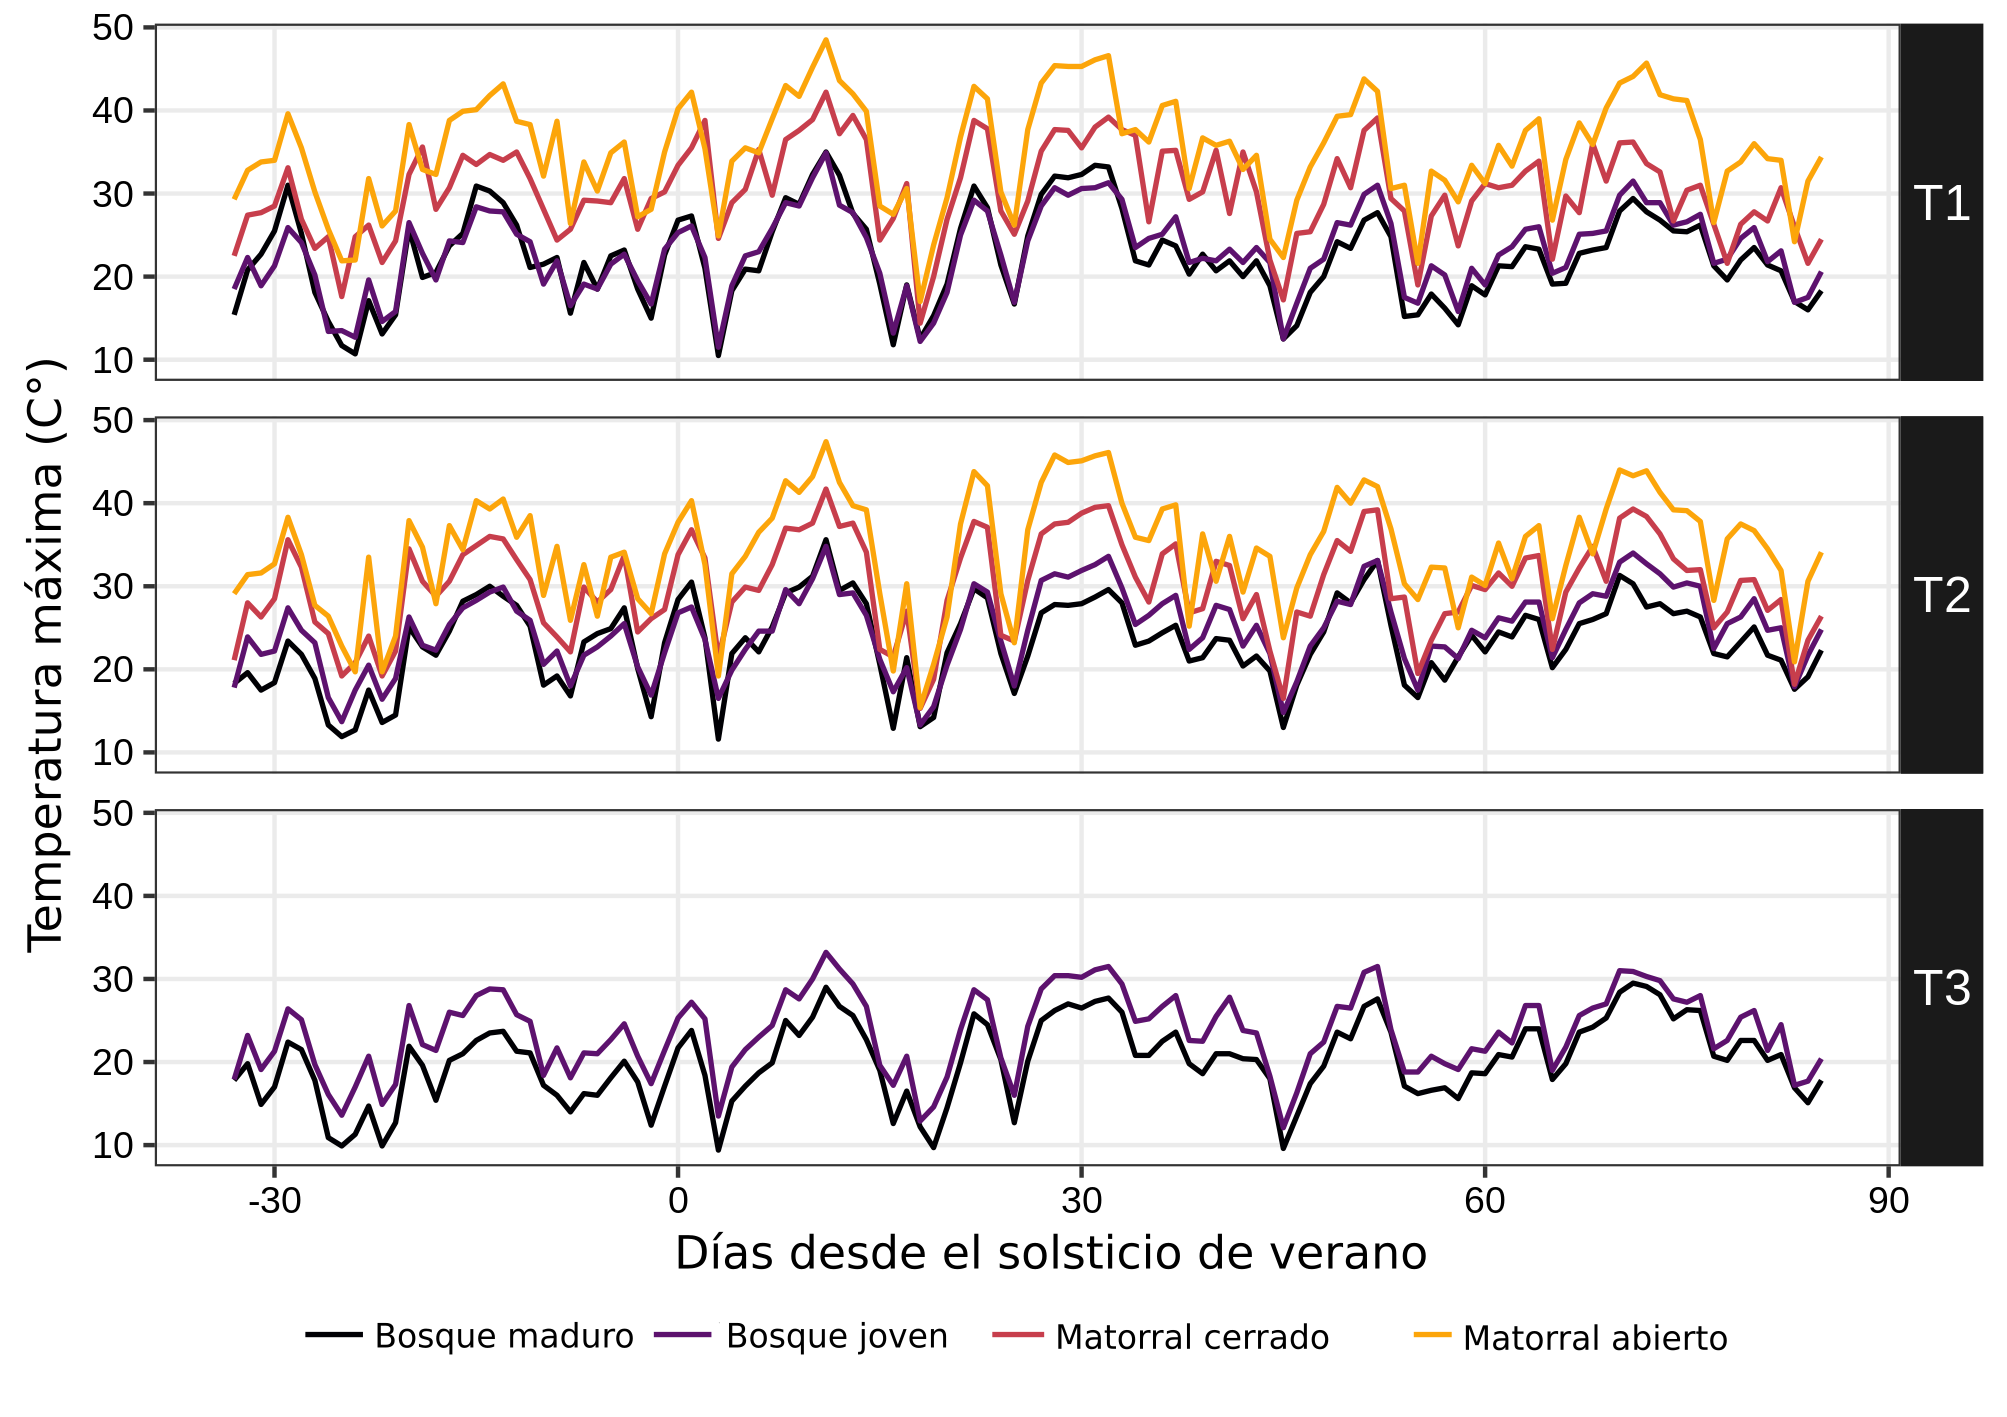
\includegraphics[width=16cm]{figuras/cap2/S07) air temperature ts.png}
    \caption[Temperatura del aire, series temporales.]{Temperatura máxima diaria (°C) a lo largo de la estación seca. El día cero corresponde al 21 de diciembre de 2019.}
    \label{fig:cap2-S07}
\end{figure}

\begin{figure}
    \centering
    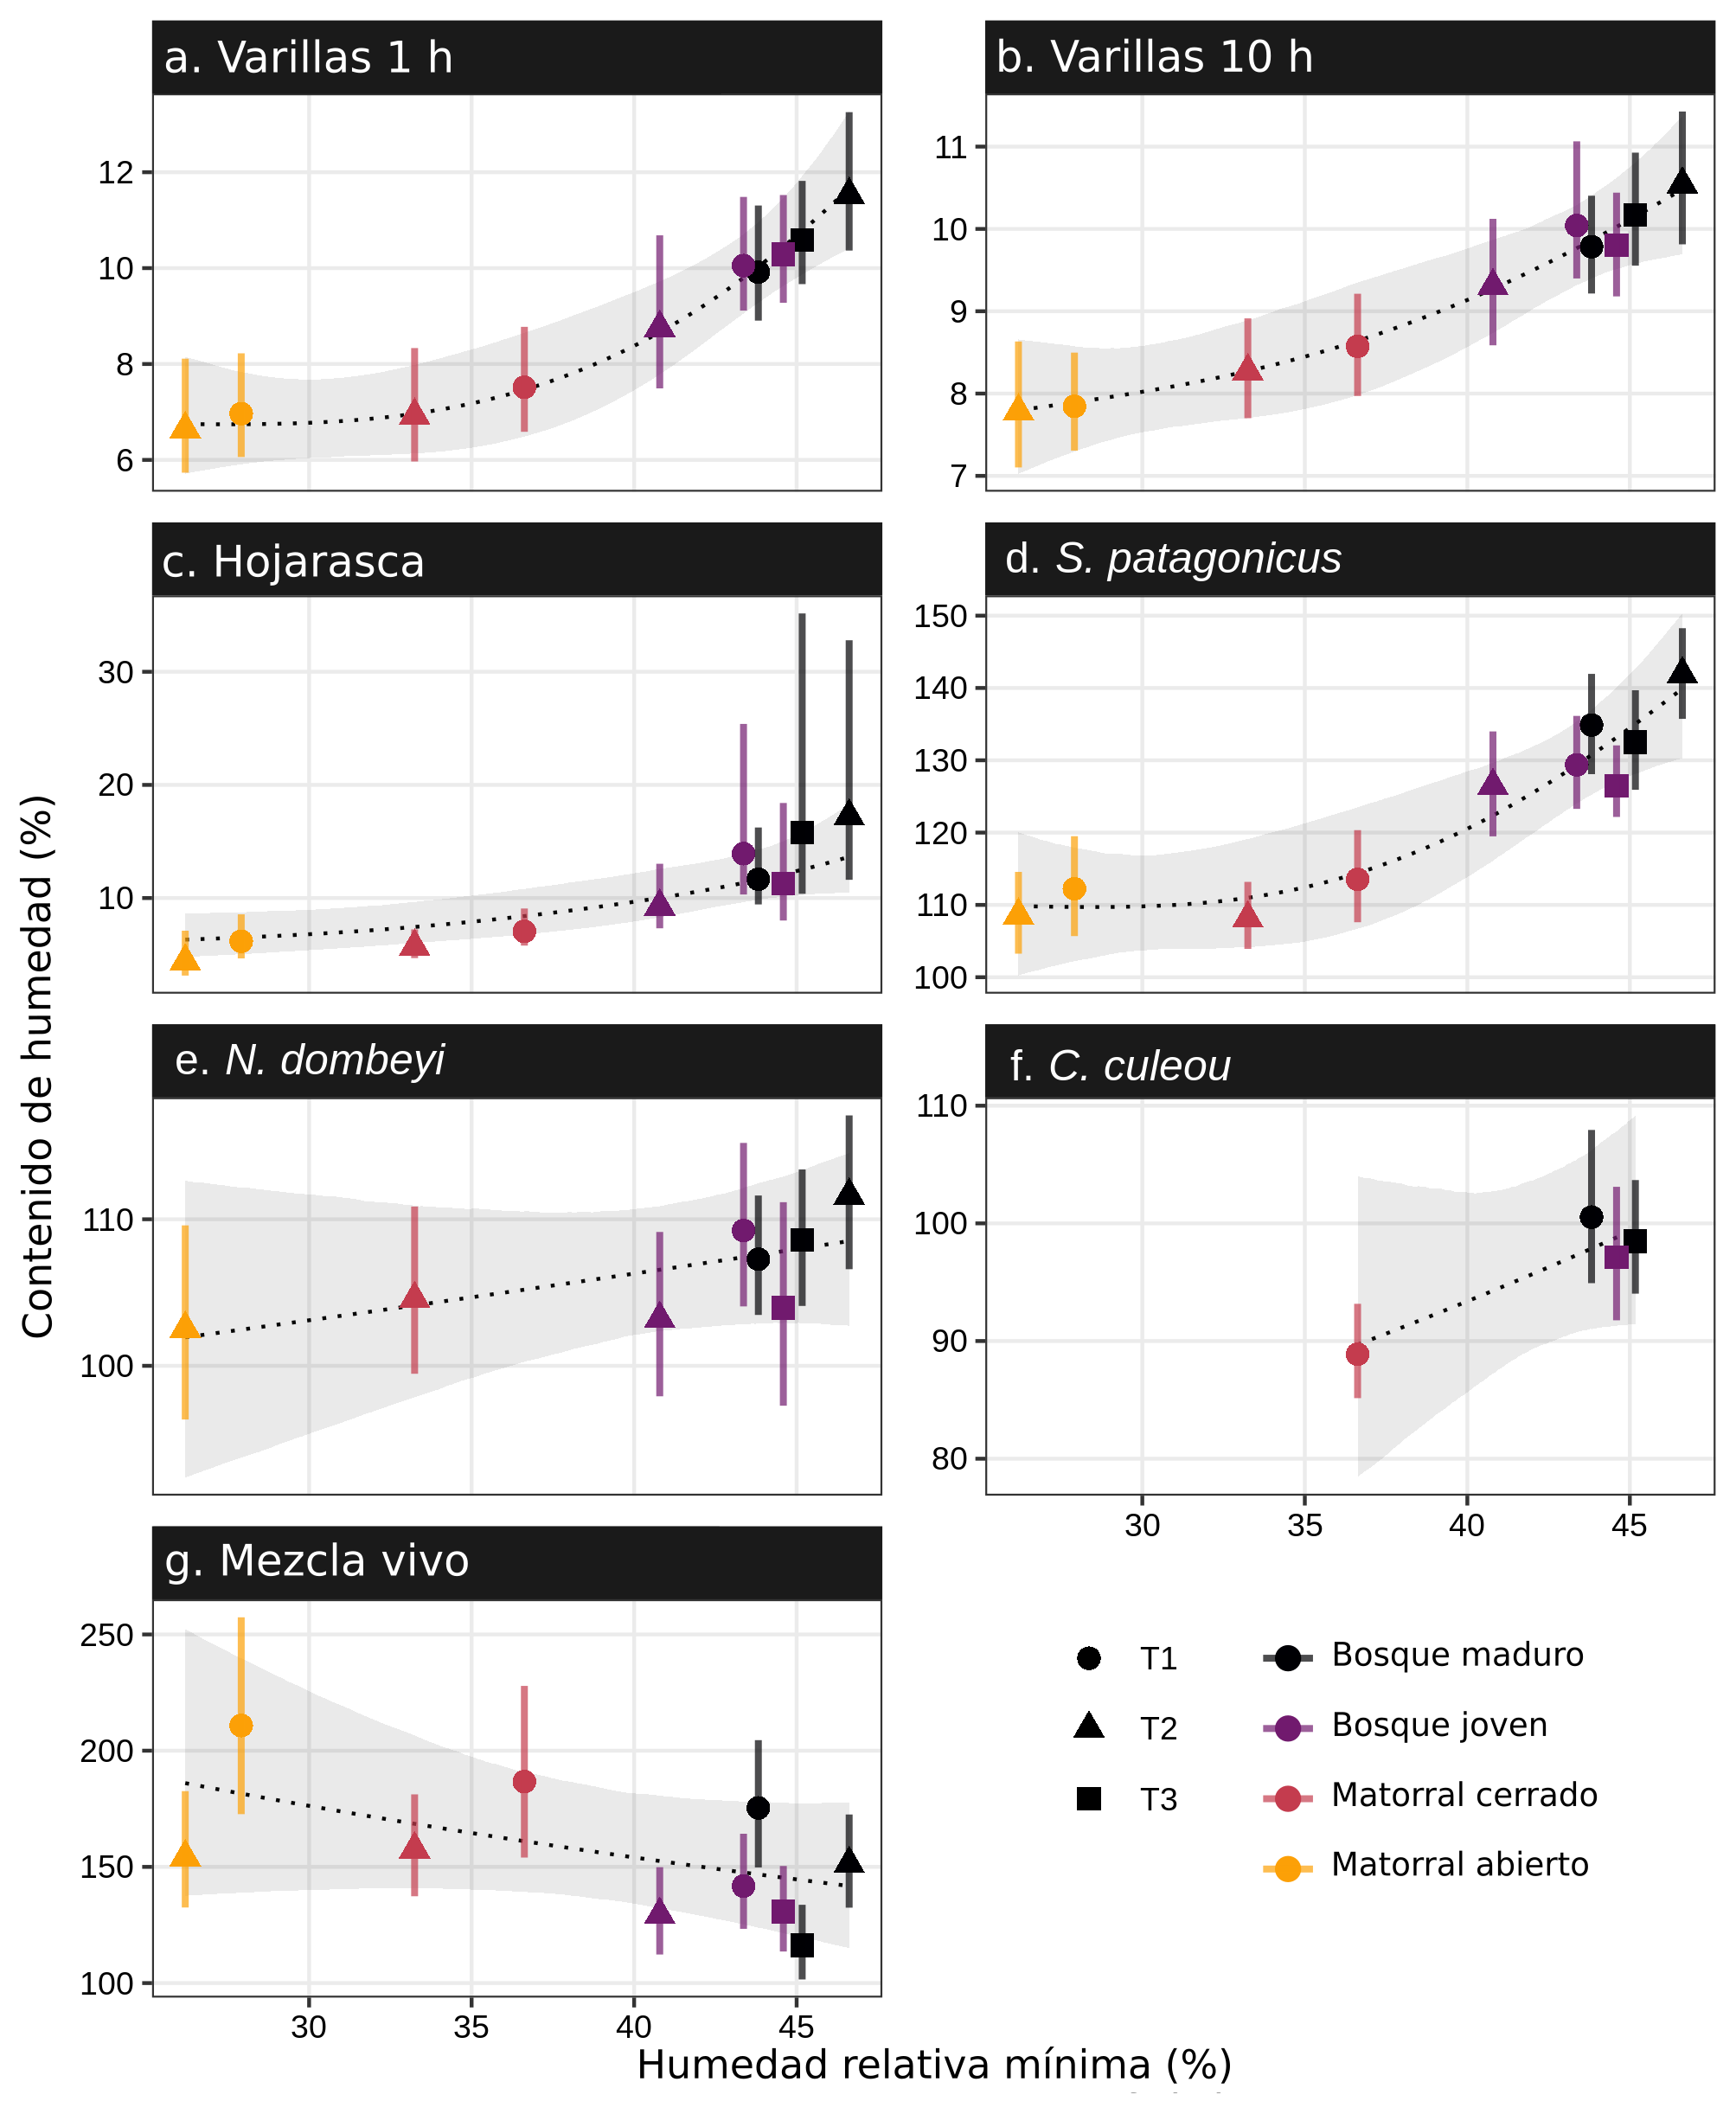
\includegraphics[width=16cm]{figuras/cap2/S08) fmc_humidity.png}
    \caption[Humedad del combustible en función de la humedad relativa del aire.]{Contenido de humedad promedio estimado en función de la humedad relativa mínima diaria promediada durante el período de estudio por sitio. Los puntos representan la media posterior para cada sitio, y las barras, los intervalos de confianza del 95\% (mismos valores que en la figura~\ref{fig:cap2-03}, panel derecho). El efecto ajustado de la temperatura se muestra con la línea discontinua (media posterior) y la banda gris (IC del 95 \%). Los modelos tuvieron la misma estructura y las mismas previas que los ajustados utilizando el DPV máximo, descritos en la Sección~\ref{cap2:humedad-methods} y en el Apéndice~\ref{append:moisture-models}.}
    \label{fig:cap2-S08}
\end{figure}

\begin{figure}
    \centering
    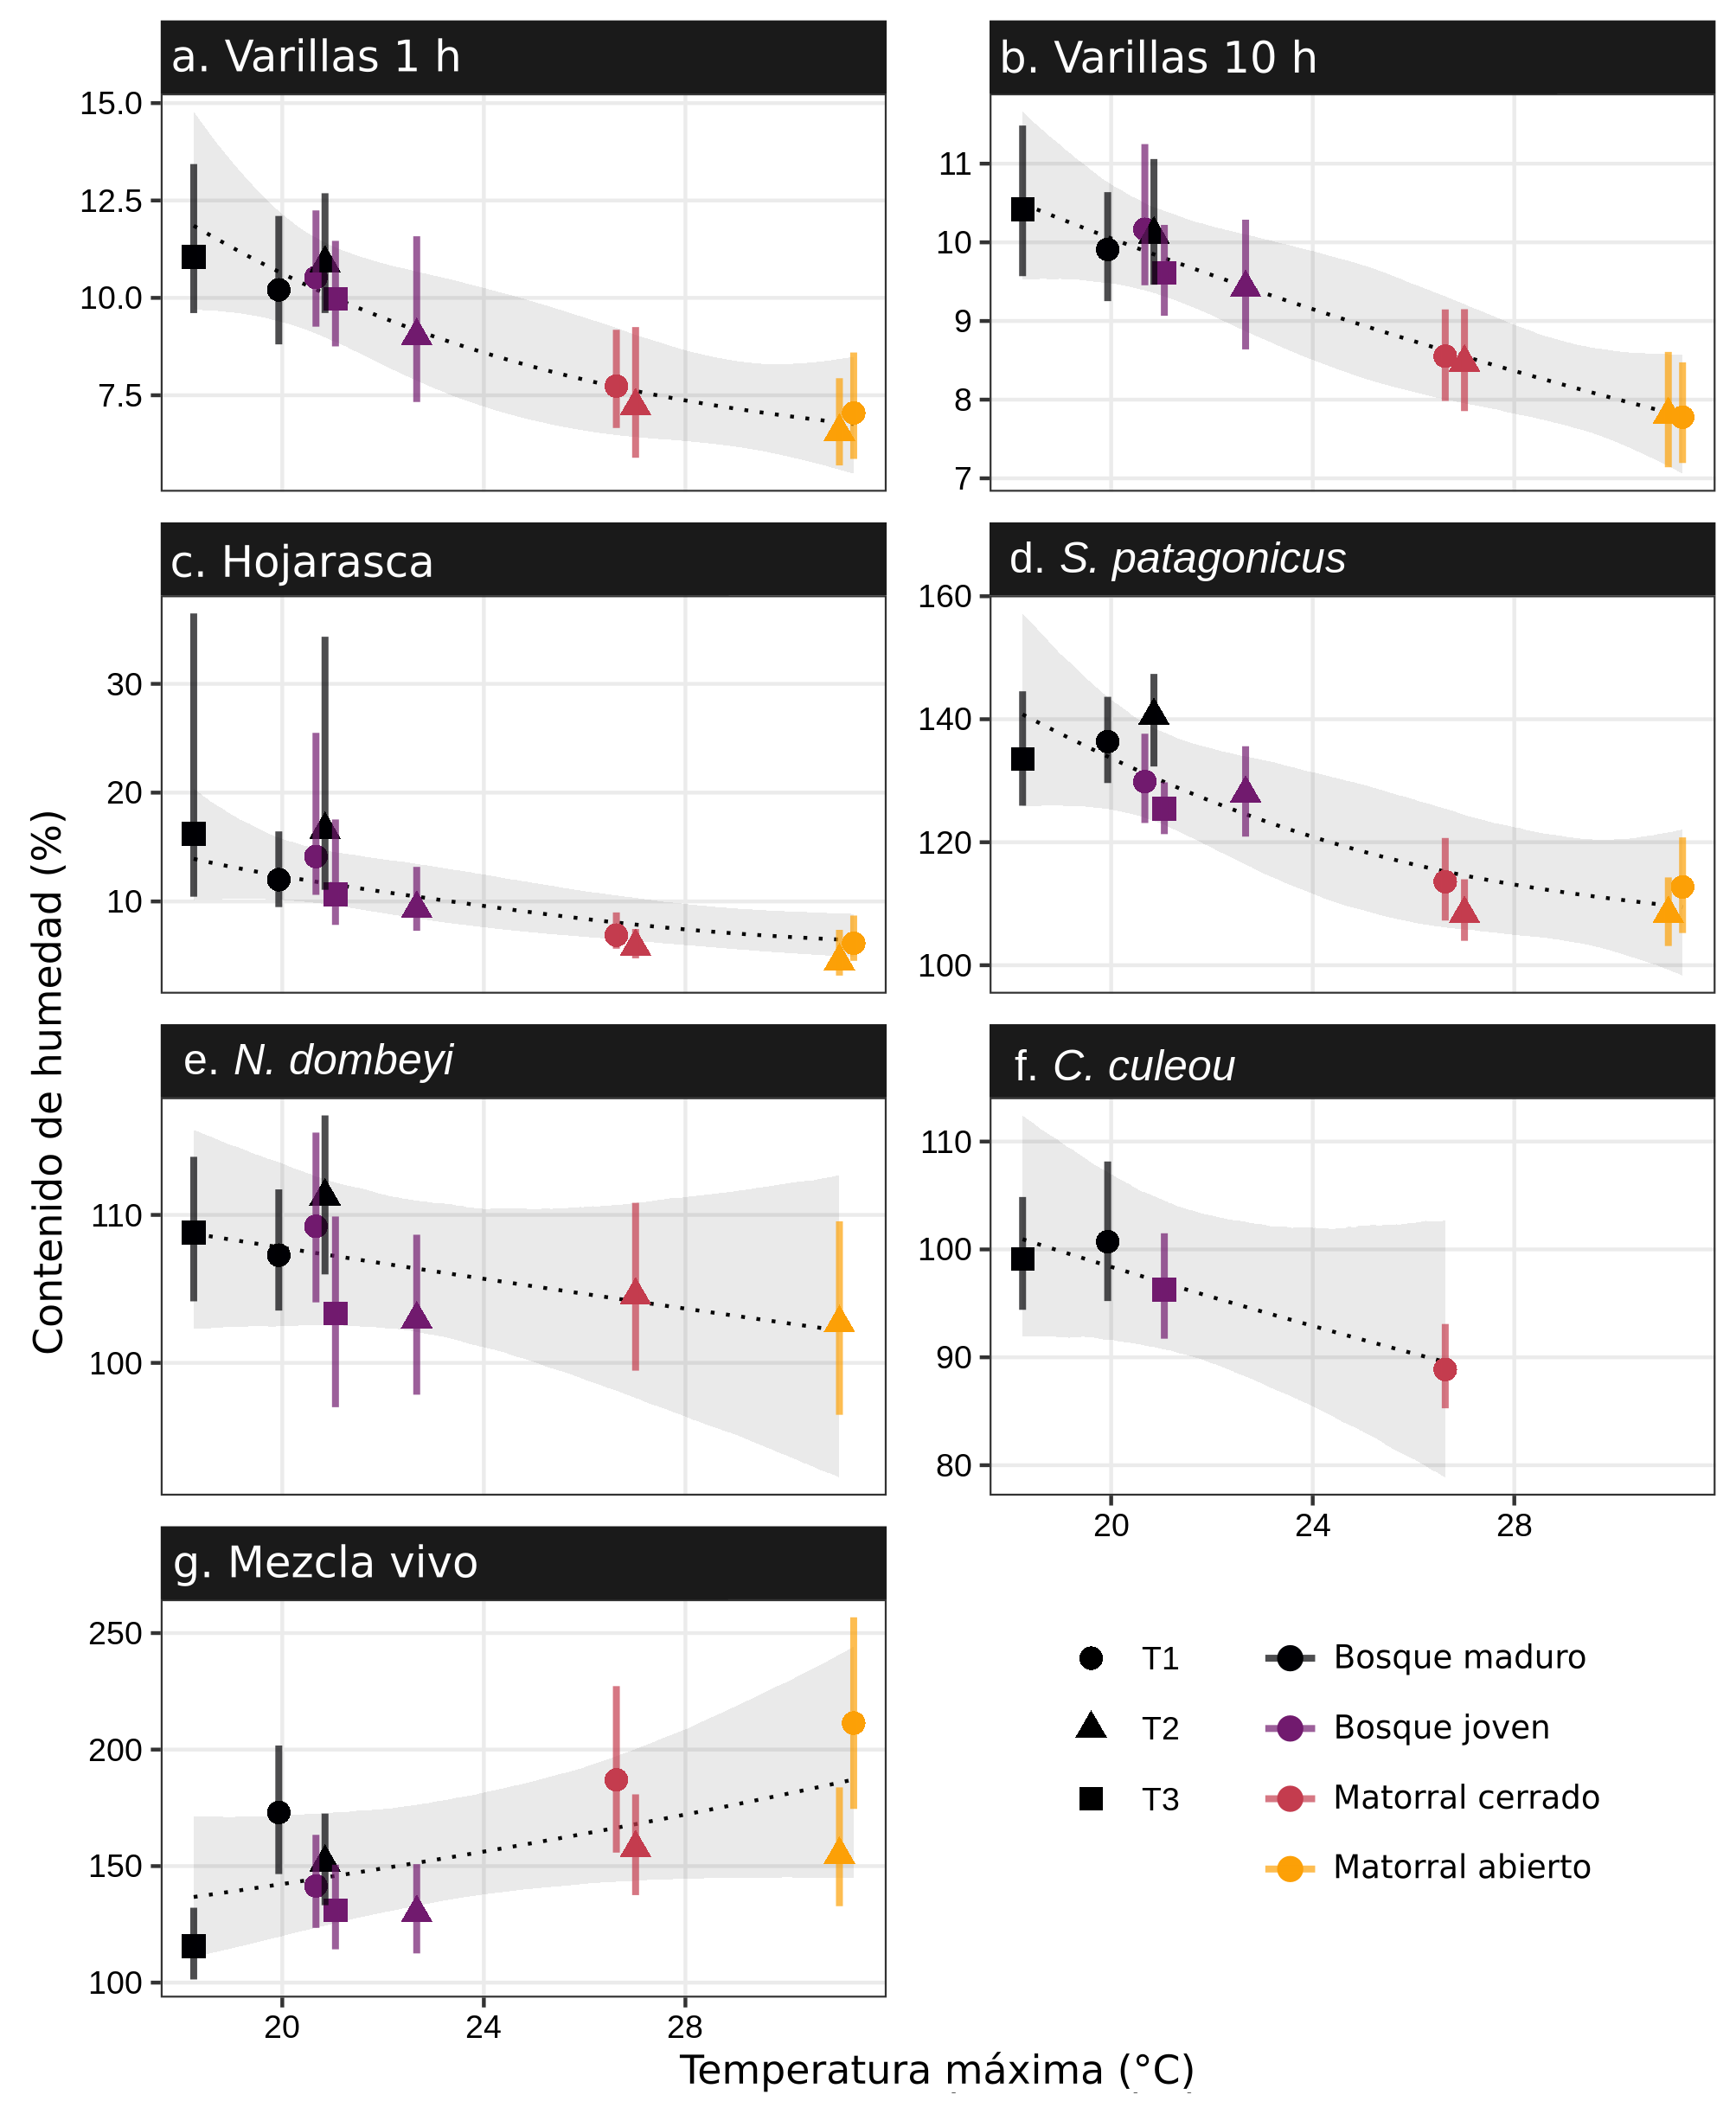
\includegraphics[width=16cm]{figuras/cap2/S09) fmc_temperature.png}
    \caption[Humedad del combustible en función de la temperatura del aire.]{Contenido de humedad promedio estimado en función de la temperatura máxima diaria promediada durante el período de estudio por sitio. Los puntos representan la media posterior para cada sitio, y las barras, los intervalos de confianza del 95 \% (mismos valores que en la figura~\ref{fig:cap2-03}, panel derecho). El efecto ajustado de la temperatura se muestra con la línea discontinua (media posterior) y la banda gris (IC del 95\%). Los modelos tuvieron la misma estructura y las mismas previas que los ajustados utilizando el DPV máximo, descritos en la Sección~\ref{cap2:humedad-methods} y en el Apéndice~\ref{append:moisture-models}.}
    \label{fig:cap2-S09}
\end{figure}

\begin{figure}
    \centering
    \caption[Humedad del combustible en función del tiempo.]{Contenido de humedad del combustible a lo largo de la estación seca por comunidad, transecta y tipo de combustible. La línea muestra el contenido de humedad promedio estimado por los GLMMs (medias posteriores), y la banda más oscura representa el intervalo de confianza del 95 \% para estas medias. Los puntos muestran los datos observados, y la banda más amplia y clara muestra el intervalo de mayor densidad del 95 \% para los datos (donde aproximadamente debería encontrarse el 95 \% de los puntos). Tratamos las fechas como un efecto aleatorio (variable categórica), pero las predicciones están conectadas con líneas para mejorar la visibilidad. (Ver figuras en las siguientes páginas).}
    \label{fig:cap2-S10-legend}
\end{figure}

\addtocounter{figure}{-1}

\begin{figure}
    \centering
    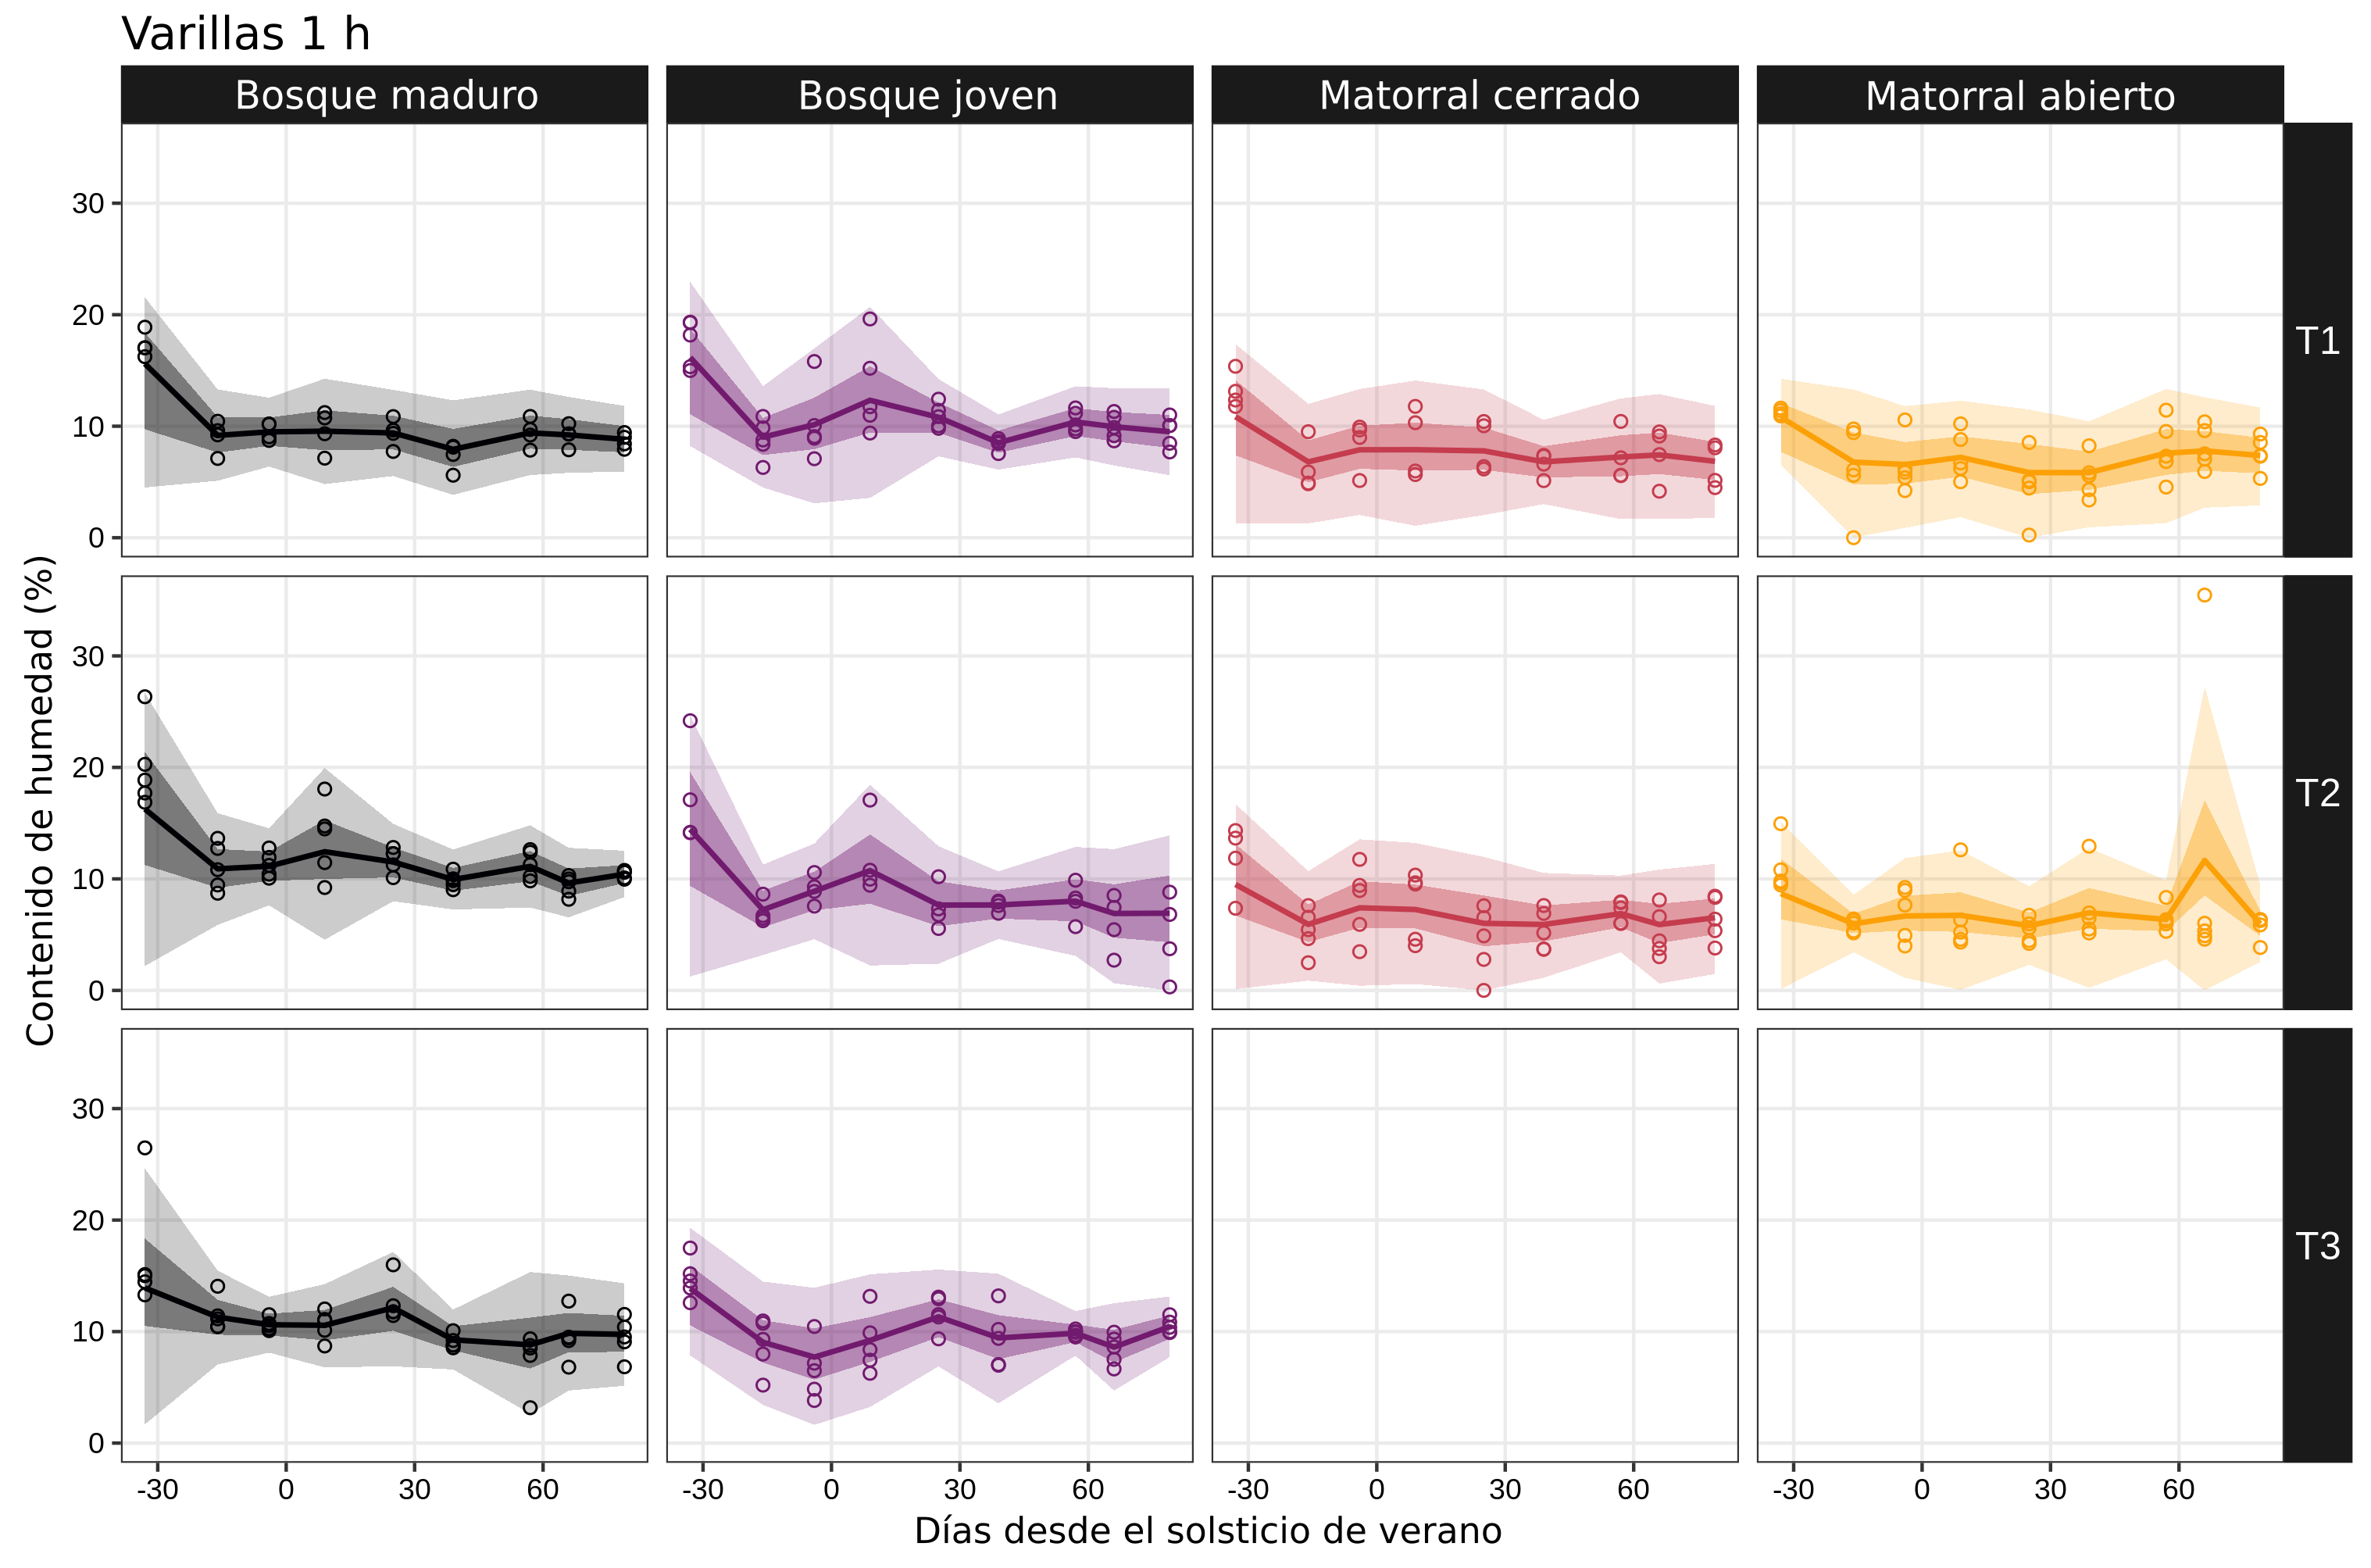
\includegraphics[width=16cm]{figuras/cap2/S10) 1h.png}
    \captionsetup{list=no}
    \caption{Ver leyenda arriba.}
    \label{fig:cap2-S10}
\end{figure}

\begin{figure}
    \centering
    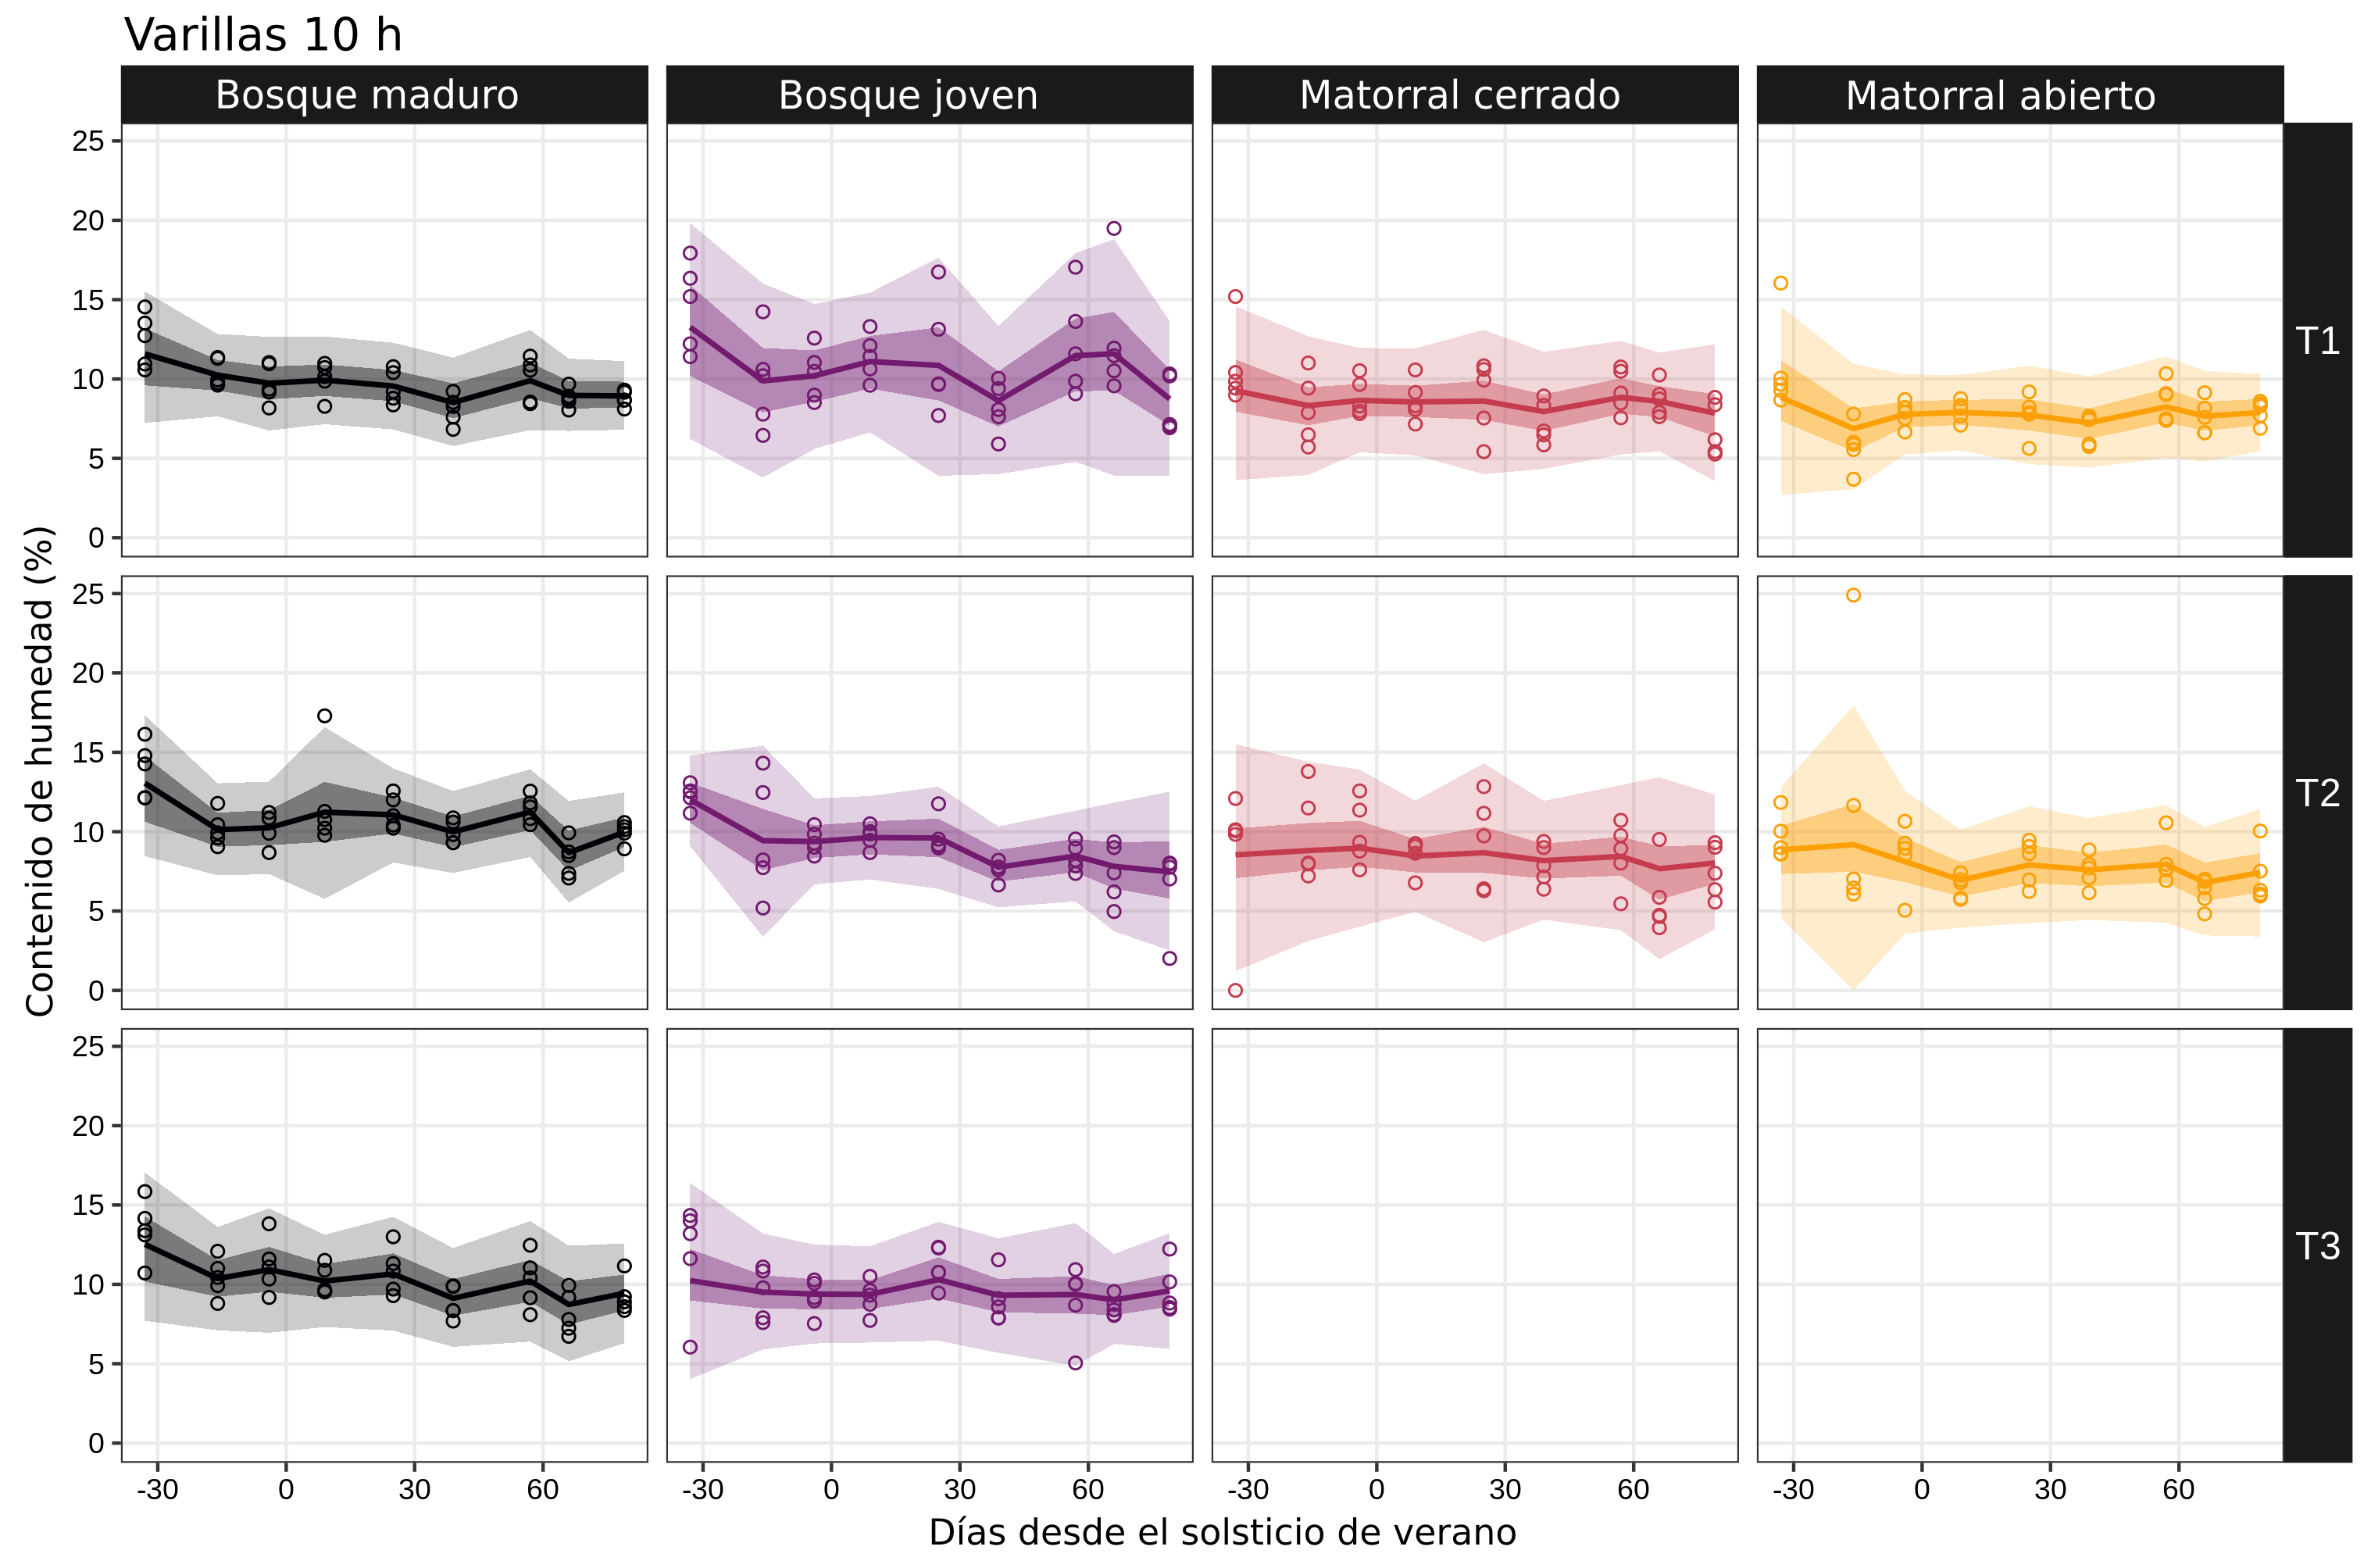
\includegraphics[width=16cm]{figuras/cap2/S11) 10 h.png}
    \captionsetup{list=no}
    \caption{Ver~\ref{fig:cap2-S10-legend}}
    \label{fig:cap2-S11}
\end{figure}

\begin{figure}
    \centering
    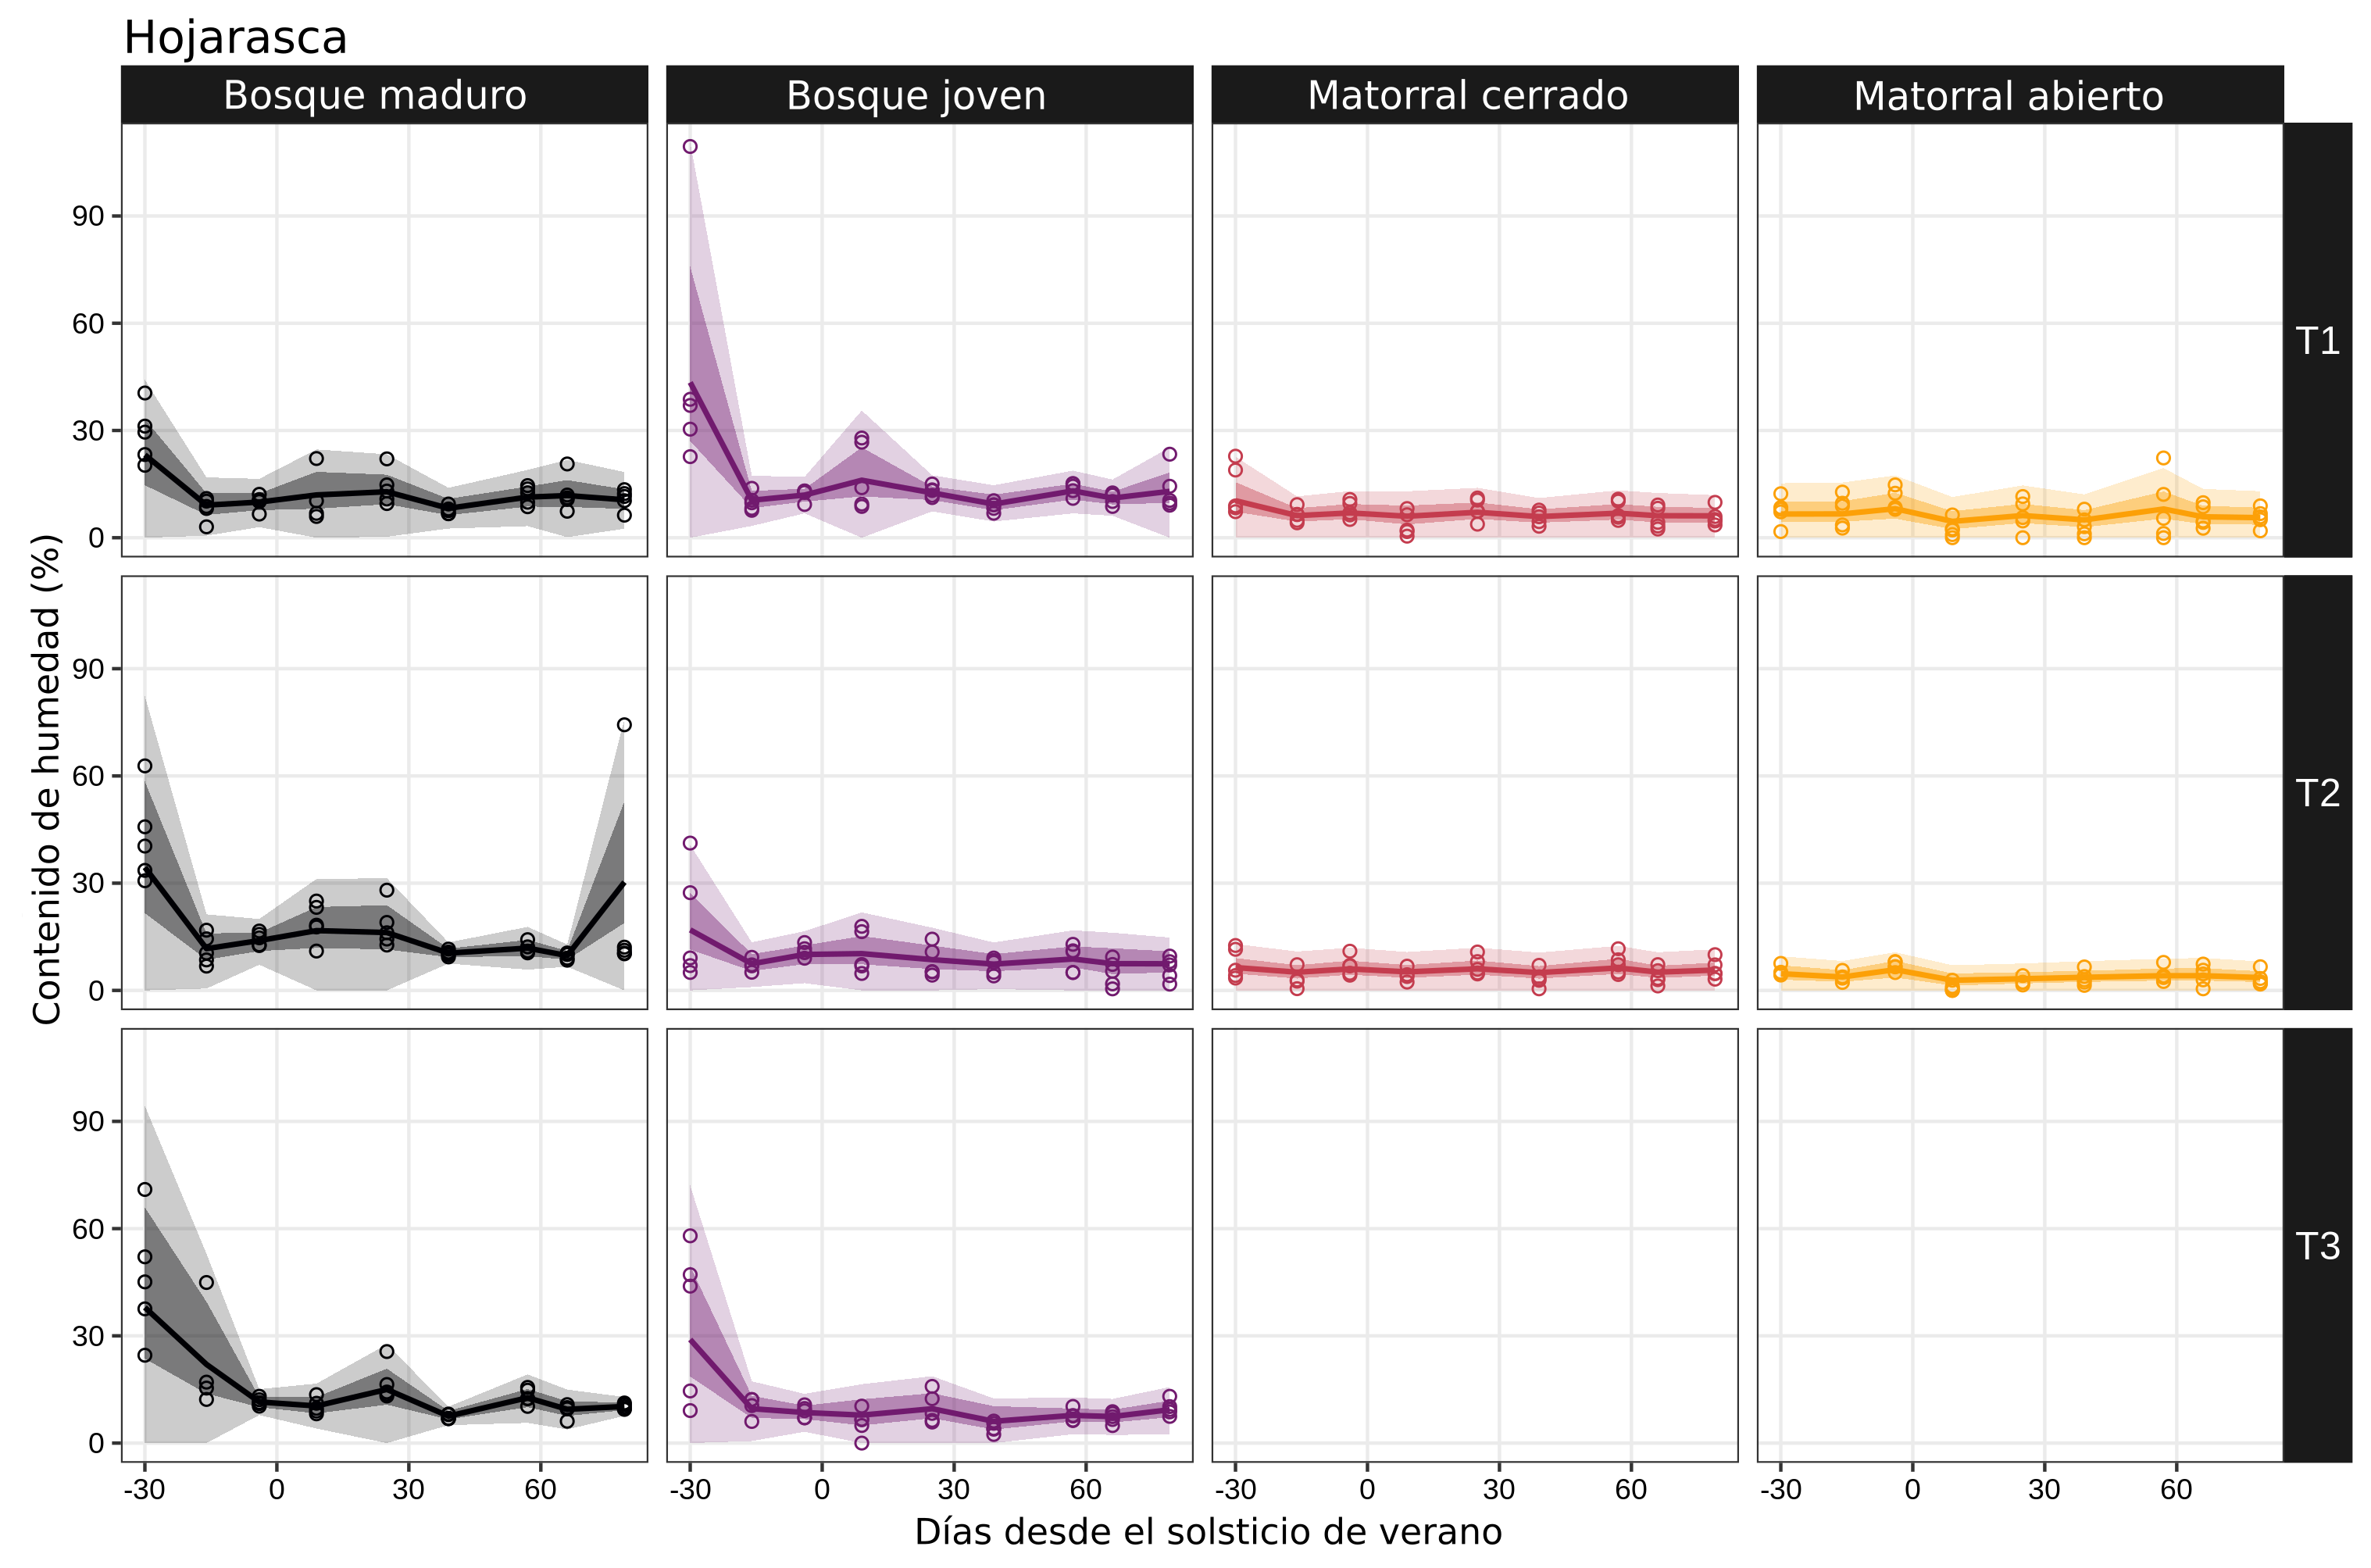
\includegraphics[width=16cm]{figuras/cap2/S12) litter.png}
    \captionsetup{list=no}
    \caption{Ver~\ref{fig:cap2-S10-legend}}
    \label{fig:cap2-S12}
\end{figure}

\begin{figure}
    \centering
    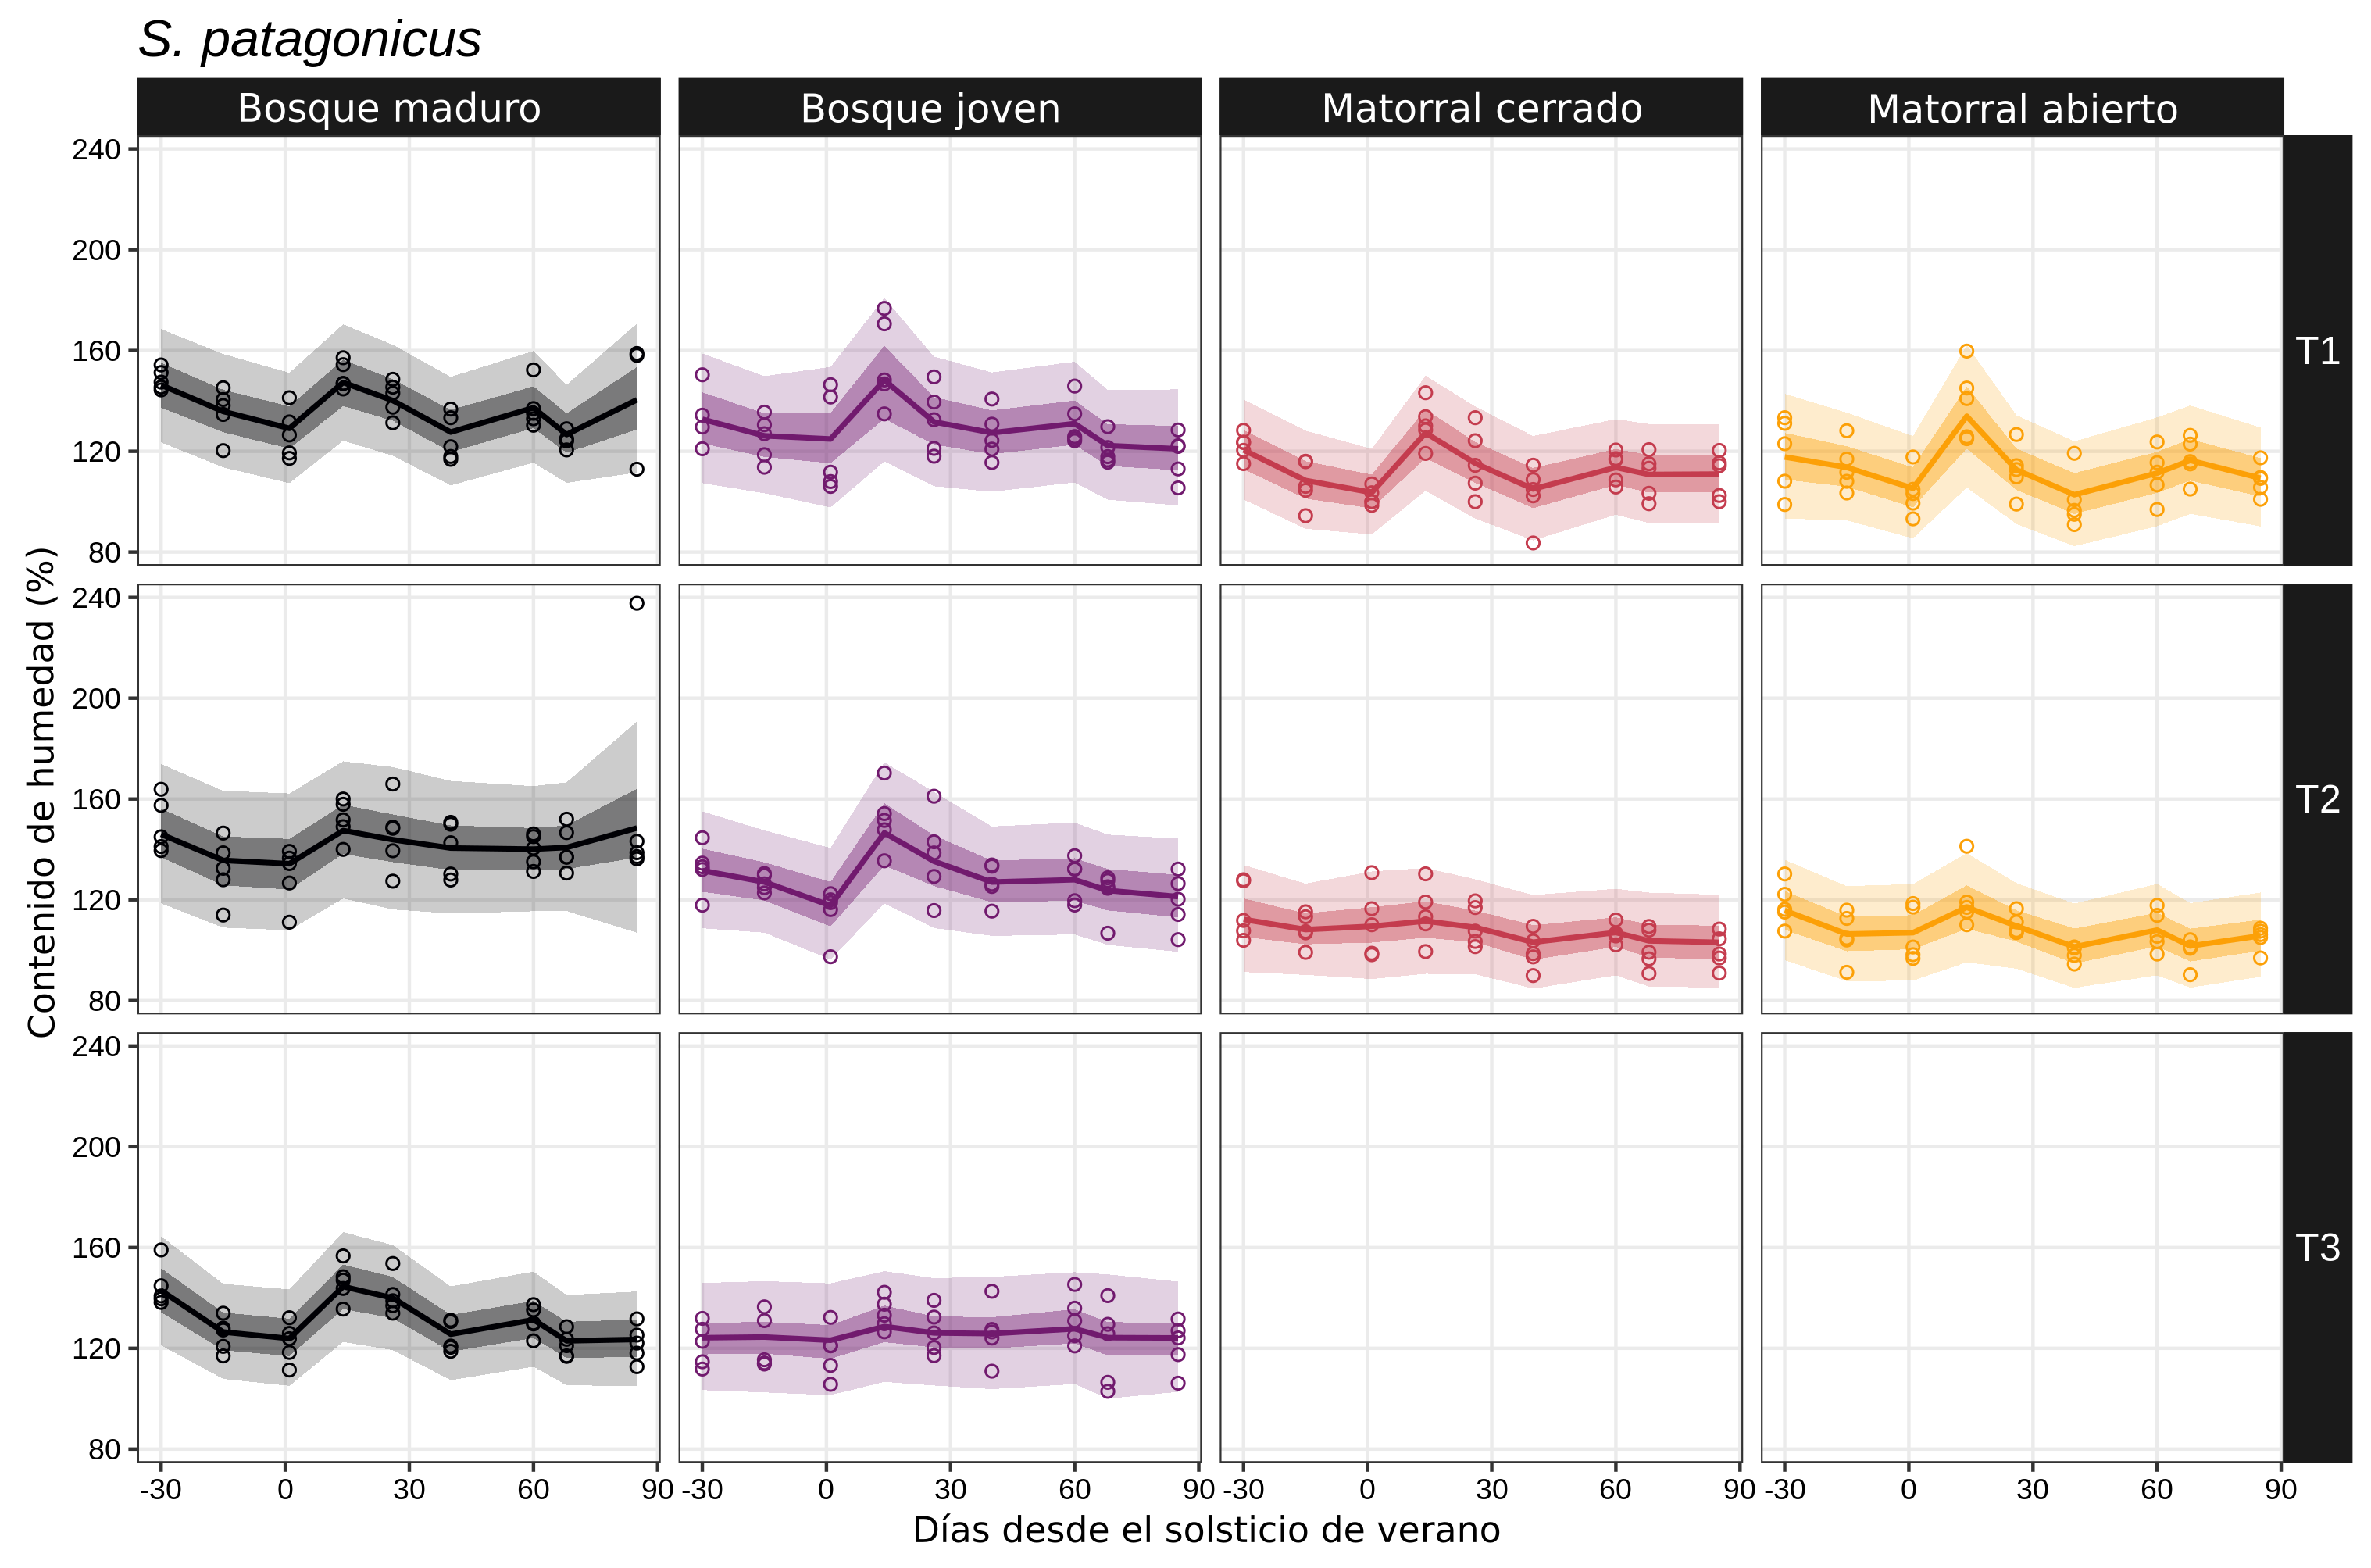
\includegraphics[width=16cm]{figuras/cap2/S13) laura.png}
    \captionsetup{list=no}
    \caption{Ver~\ref{fig:cap2-S10-legend}}
    \label{fig:cap2-S13}
\end{figure}

\begin{figure}
    \centering
    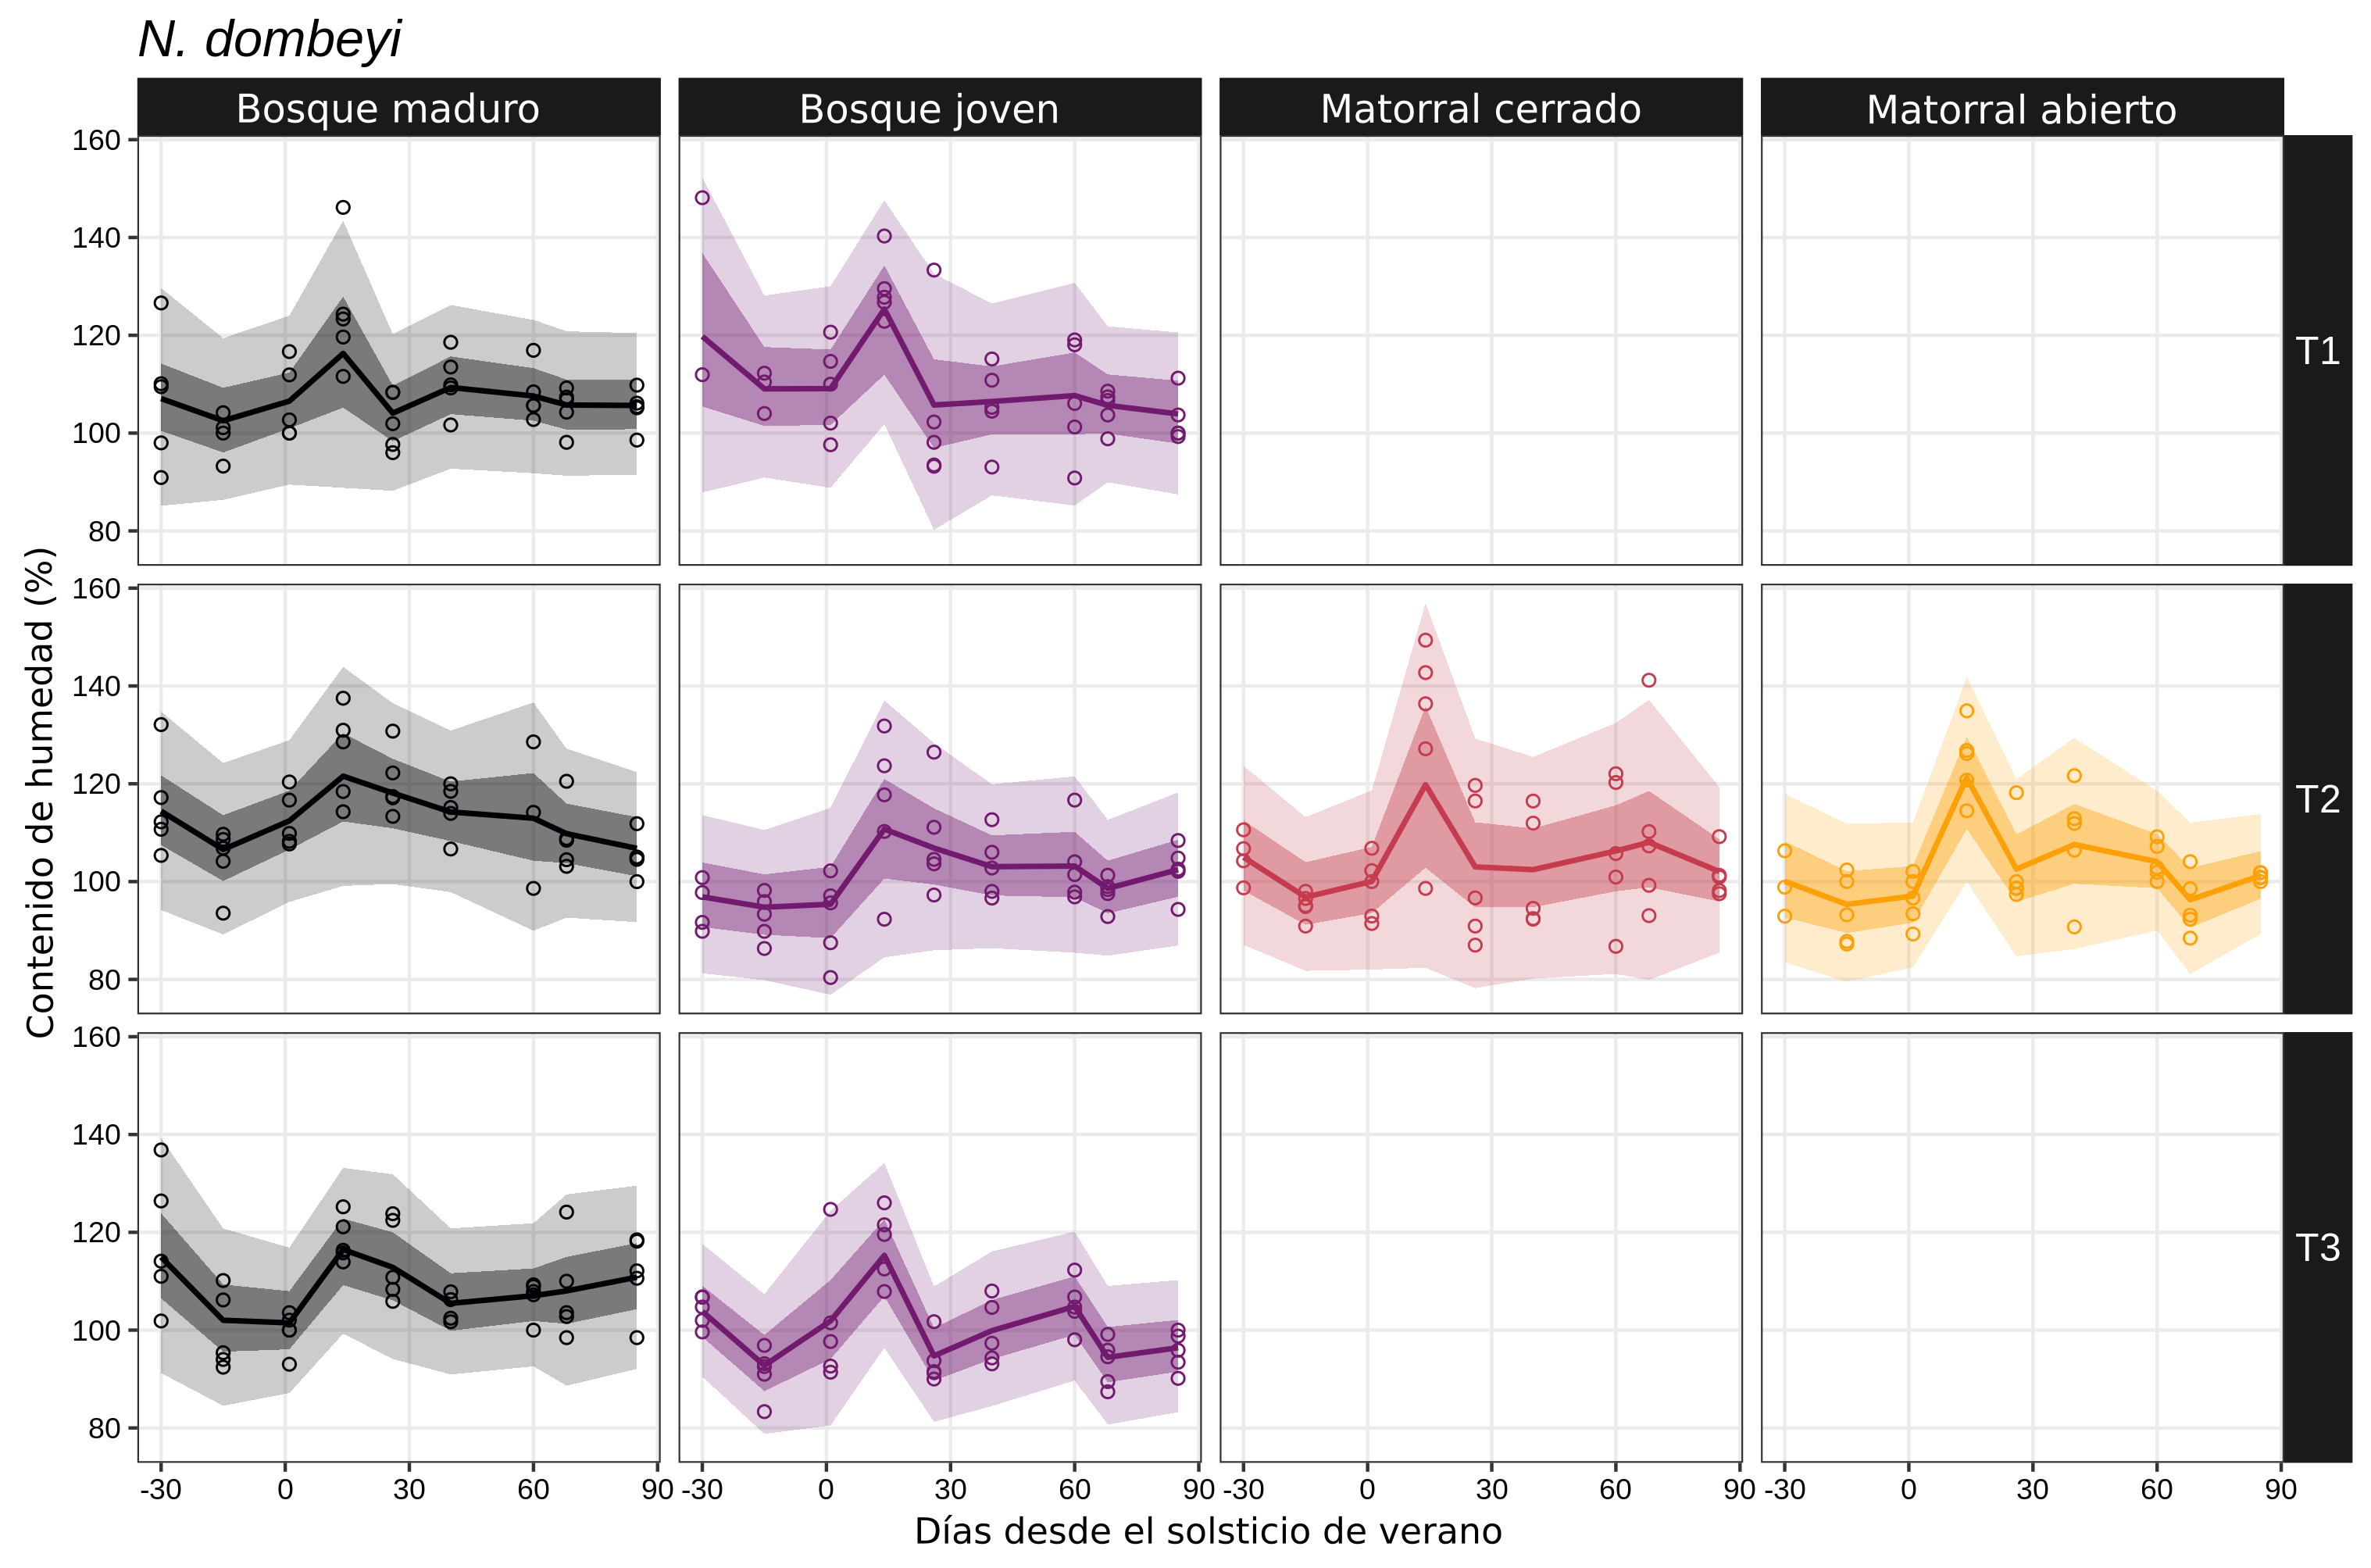
\includegraphics[width=16cm]{figuras/cap2/S14) coihue.png}
    \captionsetup{list=no}
    \caption{Ver~\ref{fig:cap2-S10-legend}}
    \label{fig:cap2-S14}
\end{figure}

\begin{figure}
    \centering
    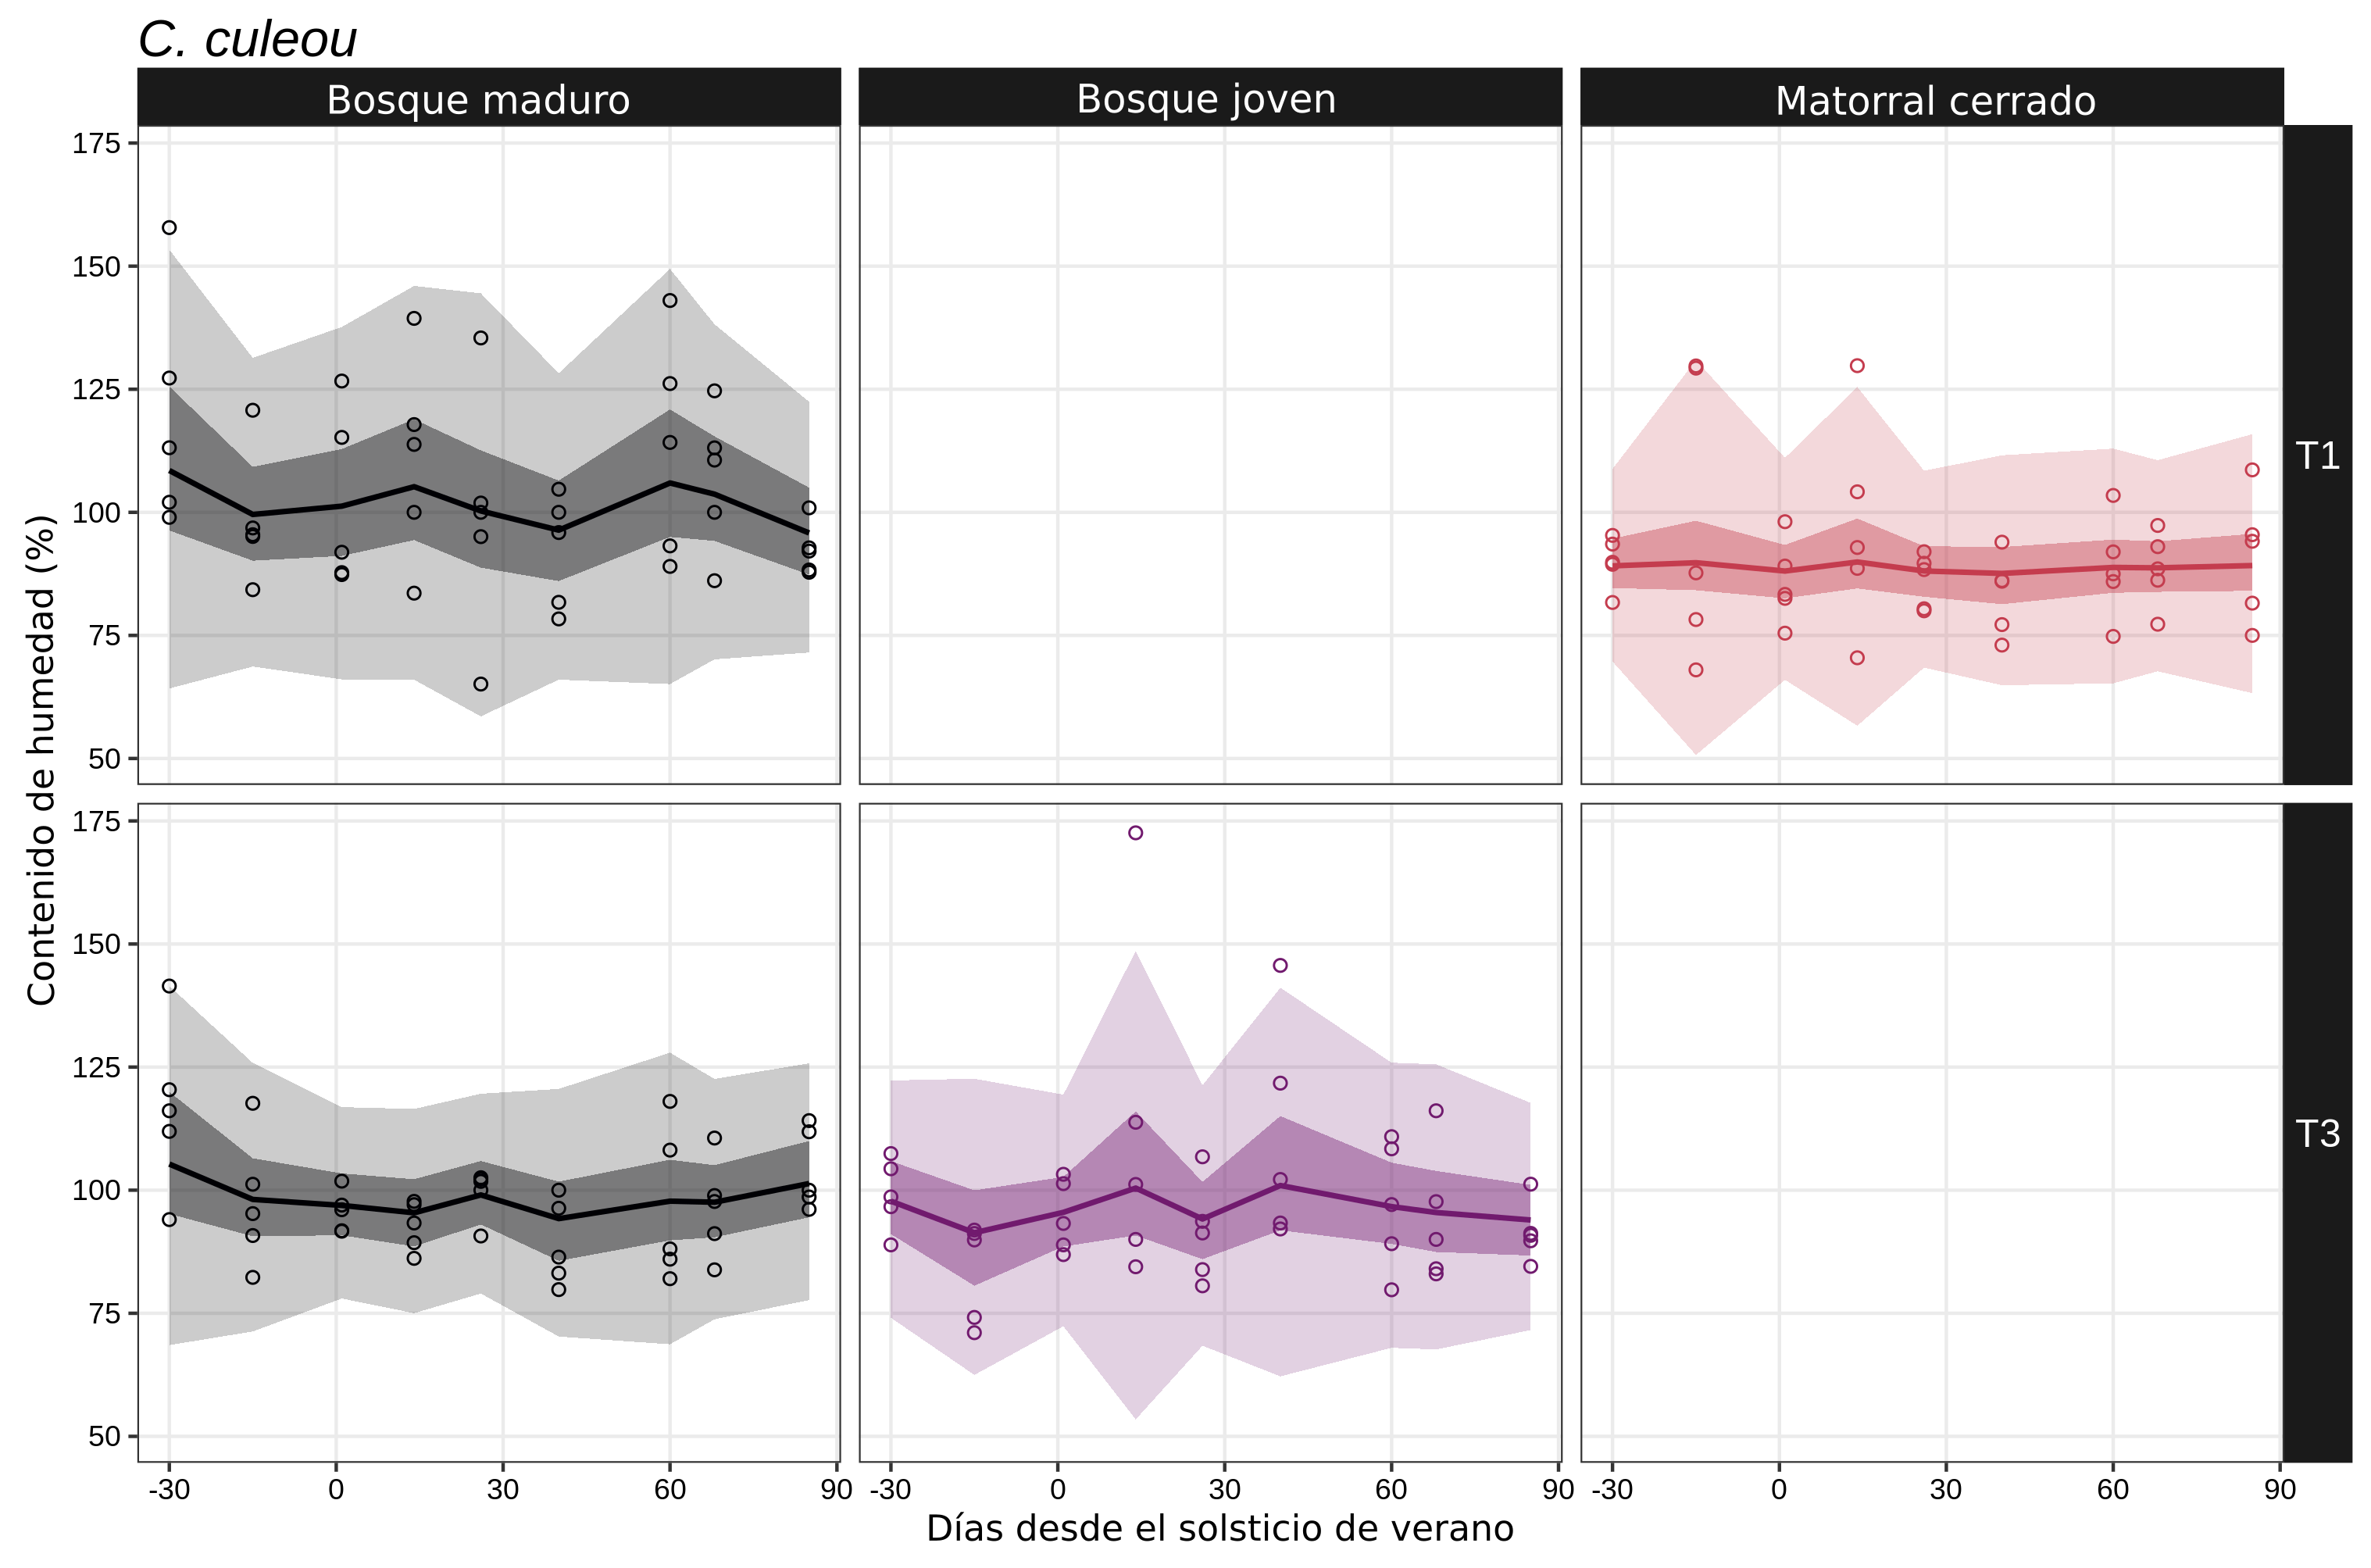
\includegraphics[width=16cm]{figuras/cap2/S15) cania.png}
    \captionsetup{list=no}
    \caption{Ver~\ref{fig:cap2-S10-legend}}
    \label{fig:cap2-S15}
\end{figure}


\begin{figure}
    \centering
    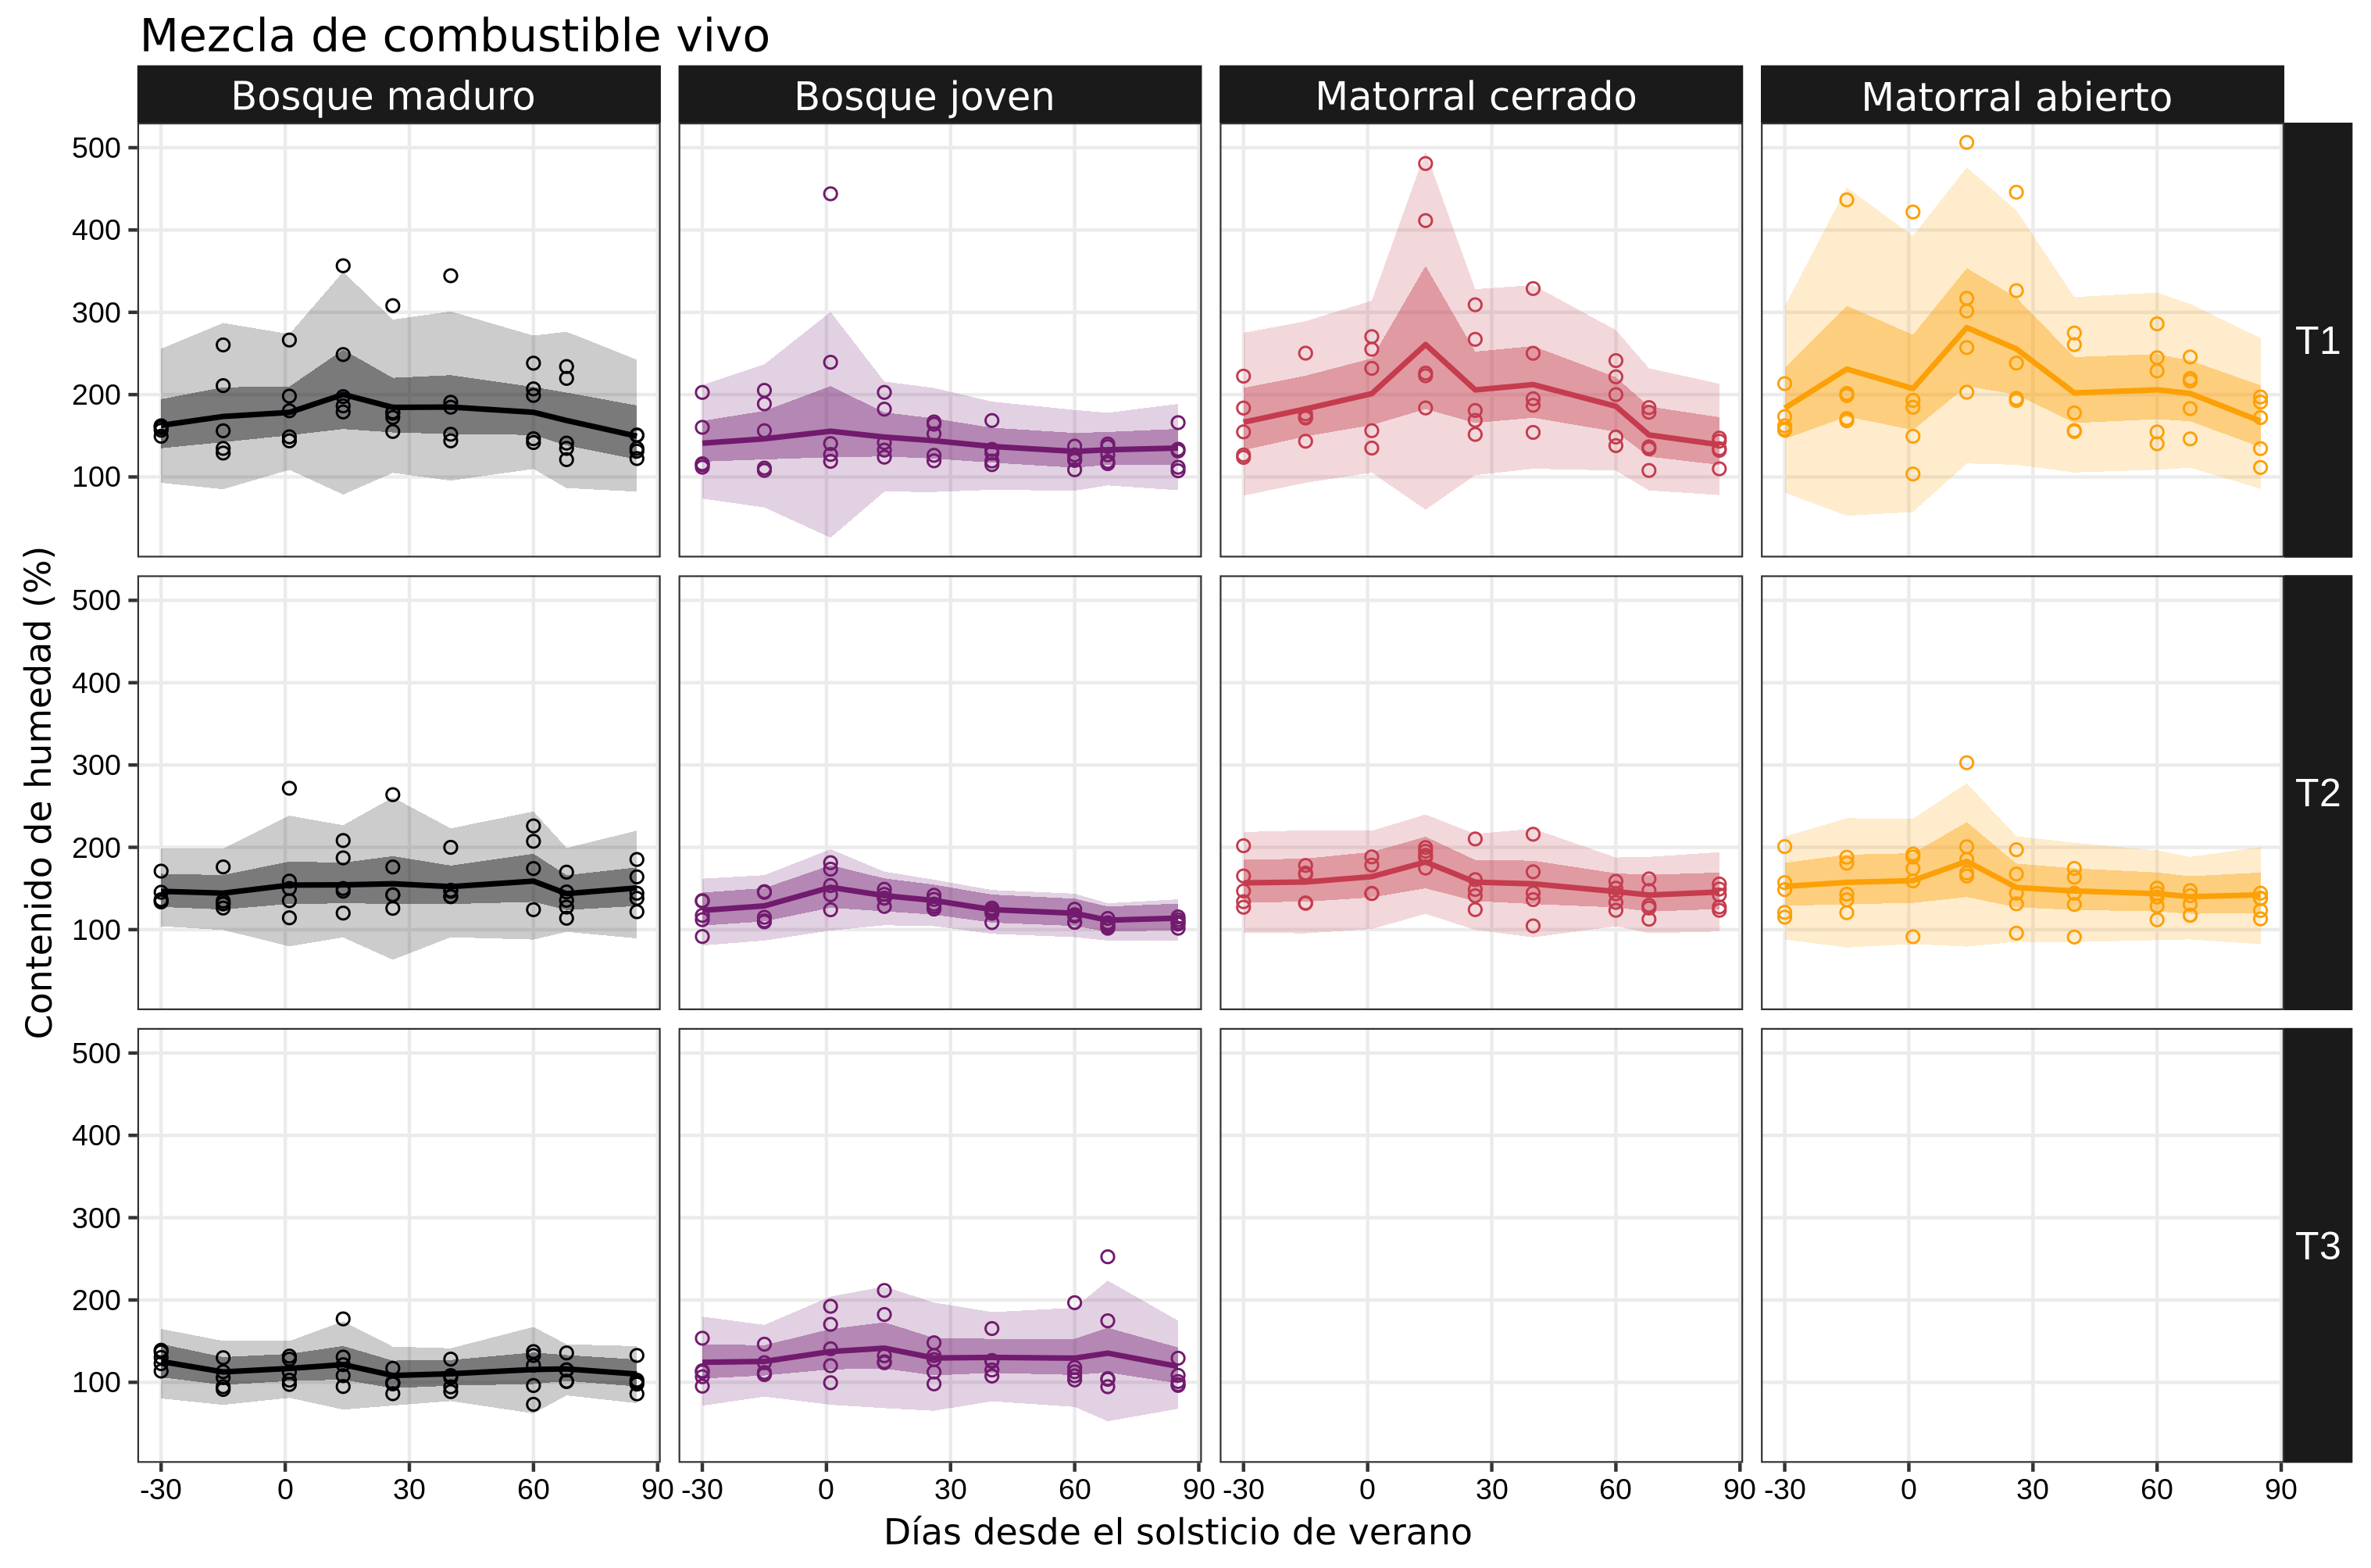
\includegraphics[width=16cm]{figuras/cap2/S16) vivos.png}
    \captionsetup{list=no}
    \caption{Ver~\ref{fig:cap2-S10-legend}}
    \label{fig:cap2-S16}
\end{figure}

\FloatBarrier

\section{Especificación completa de modelos}


\subsection{Modelo de déficit de presión de vapor}\label{append:microclimate-models}

Para comparar el DPV (Déficit de Presión de Vapor) entre comunidades dentro de cada transecta, ajustamos un modelo jerárquico asumiendo una distribución Log-Normal para las series temporales diarias de DPV y considerando la correlación temporal entre observaciones mediante una función de correlación autorregresiva de orden 1 (\texttt{corAR1}). Incluimos efectos fijos de la comunidad sobre la media ($\mu$) y el desvío estándar ($\sigma$) en la escala logarítmica, y un efecto aleatorio del sitio sobre $\mu$. 

\begin{equation}
    \begin{aligned}
    \text{log}(\textbf{y}_{cs}) &\sim \text{NMV}(\boldsymbol{\mu}_{cs}, \boldsymbol{\Sigma}_{c}) \\
    \Sigma_{c,ij} &= \sigma_{c}^{2} \ \rho^{\text{k}_{ij}} \\
    \\
    \mu_{cs} &= \eta_{c} + \delta_{s} \\
    \eta_{c} &\sim \text{Normal}(0, 5) \\
    \delta_{s} &\sim \text{Normal}(0, \tau) \\
    \tau &\sim \text{Normal}(0, 1)\text{T}[0, ] \\
    \\
    \sigma_{c} &\sim \text{Normal}(0, 1.5)\text{T}[0, ] \\
    \rho &\sim \ \text{Uniforme}(0, 1). \\
    \end{aligned}
\end{equation}
  
\noindent $\textbf{y}_{cs}$ es el vector de longitud $N = 119$ con los valores diarios máximos de DPV (entre el 18/11/2019 y el 15/03/2020) para la comunidad $c \in \{1, ..., 4\}$ y el sitio $s \in \{1, ..., 10\}$. $\text{k}_{ij}$ es la distancia temporal (en días) entre las observaciones $i$ y $j$, donde $i$ y $j \in \{1, ..., N\}$.  
$\boldsymbol{\mu}_{cs}$ es un vector que repite $\mu_{cs}$ $N$ veces, lo cual representa la mediana del DPV en la comunidad $c$ y el sitio $s$ en la escala logarítmica.  
$\sigma_{cs}$ es la desviación estándar de $\text{log}(\textbf{y}_{cs})$,  
$\rho_{cs}$ es el coeficiente de correlación temporal entre observaciones consecutivas en la escala logarítmica,  
y NMV denota una distribución Normal Multivariada.  
$\eta$ son los efectos fijos para $\mu$, que varían entre comunidades, mientras que $\delta$ son efectos aleatorios a nivel de sitio. 
  
La distribución Normal está parametrizada con media y desvío estándar. T[,] indica distribuciones truncadas en los valores indicados por el intervalo, donde un valor faltante indica $\pm \ \infty$. Como la respuesta asume Log-Normal, su media se calcula como:

\[
\text{E}(\textbf{y}_{cs}) = \text{exp}\left(\mu_{cs} + \frac{\sigma_{cs}^2}{2}\right),
\]

mientras que:

\[
\text{exp}(\mu_{cs}) = \text{mediana}(\textbf{y}_{cs}).
\]

Corrimos 10 cadenas markovianas durante 2000 iteraciones, dejando 1000 para la fase de calentamiento. Considerando todos los parámetros y cantidades derivadas calculadas en Stan (e.g., medias), el valor máximo de $\hat{\text{R}}$ fue 1.003, lo que indica convergencia, y el tamaño efectivo de muestra más pequeño fue 2408.  

\subsection{Modelos de humedad del combustible}\label{append:moisture-models}

Dado que nos interesaba la variación en el contenido de humedad entre comunidades mediada por el microclima, ajustamos un Modelo Lineal Generalizado Mixto (GLMM, por sus siglas en inglés) para cada tipo de combustible, especificando una regresión del contenido de humedad en función del DPV (Déficit de Presión de Vapor) a nivel de sitio, utilizando como predictora el promedio diario máximo de DPV de cada sitio. Modelamos la media de la respuesta con un enlace log, incluyendo efectos aleatorios de sitio (combinaciones de comunidad y transecta), fecha y su combinación. Inicialmente intentamos ajustar una estructura de correlación temporal para los efectos aleatorios de la fecha, pero con solo nueve fechas no pudimos estimar el parámetro de correlación, por lo que asumimos efectos independientes. No incluimos el factor comunidad en los modelos porque suponíamos que el mayor efecto de la comunidad sobre el contenido de humedad estaría mediado por el microclima y porque la comunidad y el DPV están altamente correlacionados, lo que habría dificultado la estimación del efecto del DPV y la interpretación de los resultados.  

Para los combustibles vivos asumimos una distribución Gamma, ya que su asimetría permitió un buen ajuste a los datos. En el caso de los combustibles muertos, se observaron valores extremos del contenido de humedad cercanos a cero, lo que llevaba a la distribución Gamma a estimar una varianza alta para acomodar estos valores bajos, implicando también una alta densidad en valores de contenido de humedad elevados que no eran compatibles con los datos. Esto nos llevó a preferir distribuciones Normales truncadas en 0 para el contenido de humedad de los combustibles muertos, lo que permite una mayor densidad en valores cercanos a cero sin ajustar una varianza extrema.  

A continuación especificamos completamente el modelo para la mezcla de combustibles vivos, que fue el más complejo, y mencionamos las diferencias para otros tipos de combustible más abajo.  

\[
\begin{aligned}
    \text{y}_{dsp} &\sim \text{Gamma}(\alpha_{ds}, \beta_{dsp})\\
    \alpha_{ds} &= \frac{1}{\phi_{ds}}\\
    \beta_{dsp} &= \frac{1}{\mu_{dsp} \ \phi_{ds}}.\\
\end{aligned}
\]

\noindent Aquí, $\text{y}_{dsp}$ es el contenido de humedad en la fecha $d \in \{1, ..., 9\}$, sitio $s \in \{1, ..., 10\}$ y parcela de muestreo $p \in \{1, ..., 50\}$ (había 5 parcelas de muestreo por sitio). $\alpha$ y $\beta$ son los parámetros de forma y tasa, donde $\mu = \text{E}(\text{y})$, y $\phi$ es un parámetro de dispersión. Modelamos tanto $\mu$ como $\phi$ con una función de enlace log.  

Modelo para $\mu$:
  
\begin{equation}
    \begin{aligned}
    \text{log}(\mu_{dsp}) &= \eta_\mu + \lambda \ \text{DPV}_s + \varepsilon_{\mu \text{S}, s} + \varepsilon_{\mu \text{DS}, ds} + \varepsilon_{\mu \text{P}, p}\\
    \\
    \eta_{\mu} &\sim \text{Normal}(\text{log}(\text{media previa}_{\eta \mu}), 1) \\
    \lambda &\sim \text{Normal}(0, 1) \\
    \\
    \varepsilon_{\mu \text{S}, s} &\sim \text{Normal}(0, \sigma_{\mu \text{S}}) \\ 
    \sigma_{\mu \text{S}} &\sim \text{Normal(0, 1)\text{T}[0, ]} \\
    \\
    \varepsilon_{\mu \text{DS}, ds} &\sim \text{Normal}(0, \sigma_{\mu \text{DS,s}}) \\
    \sigma_{\mu \text{DS,s}} &\sim \text{Normal}(0, 0.7)\text{T}[0, ] \\
    \end{aligned}
\end{equation}

\noindent El sufijo $\mu$ indica que estos parámetros modelan $\mu$ y no $\phi$. Los subíndices en minúscula ($d,\ s$ y $p$) son variables, mientras que los subíndices en mayúscula (S, DS y P) se usan para nombrar los efectos aleatorios y los desvíos estándar correspondientes al sitio, fecha $\times$ sitio y parcela, respectivamente. $\varepsilon_{\mu \text{DS}, ds}$ es un efecto aleatorio para la fecha dentro de cada sitio, donde cada sitio tiene su propio desvío estándar entre fechas: $\sigma_{\mu \text{DS},s}$.  
$\text{DPV}_s$ es el promedio diario máximo de DPV en cada sitio. El valor de $\text{media previa}_{\eta \mu}$ varió entre tipos de combustible (ver Tabla~\ref{tab:cap2-S02}).  
  
El modelo para $\phi$ fue similar, excluyendo únicamente el efecto del DPV y estimando solo un $\sigma_{\phi \text{DS}}$ (este parámetro varió por sitio solo en el modelo de hojarasca):  

\begin{equation}
    \begin{aligned}
    \text{log}(\phi_{dsp}) &= \eta_\phi + \varepsilon_{\phi \text{S}, s} + \varepsilon_{\phi \text{DS}, ds}\\
    \\
    \eta_{\phi} &\sim \text{Normal}(\text{log}(\text{media previa}_{\eta \phi}), 1) \\
    \\
    \varepsilon_{\phi \text{S}, s} &\sim \text{Normal}(0, \sigma_{\phi \text{S}}) \\ 
    \sigma_{\phi \text{S}} &\sim \text{Normal}(0, 1)\text{T}[0, ] \\
    \\
    \varepsilon_{\phi \text{DS}, ds} &\sim \text{Normal}(0, \sigma_{\phi \text{DS}}) \\
    \sigma_{\phi \text{DS}} &\sim \text{Normal}(0, 1)\text{T}[0, ]
    \end{aligned}    
\end{equation}

El efecto aleatorio para las parcelas de muestreo se incluyó únicamente para la mezcla de combustibles vivos, ya que los modelos de combustibles muertos no convergieron cuando se agregó este término, probablemente porque el efecto de la parcela era demasiado pequeño para los combustibles muertos, como lo mostró el análisis de residuos. En el caso de los combustibles vivos de una sola especie, no registramos los individuos muestreados, por lo que no contamos con una variable análoga a la parcela de muestreo. El valor de $\text{media previa}_{\eta \phi}$ varió entre tipos de combustible (ver Tabla~\ref{tab:cap2-S02}).

En el caso de los combustibles muertos, la verosimilitud fue una distribución Normal truncada por abajo en cero y desvío estándar $\phi$:  

\[
\text{y}_{dsi} \sim \text{Normal}(\mu_{ds}, \phi_{ds})\text{T}[0, ],
\]

\noindent y los modelos para $\text{log}(\mu)$ y $\text{log}(\phi)$ se especificaron de manera similar a los de la mezcla de combustibles vivos. (Aquí no hay parcelas de muestreo, pero hay alrededor de 5 observaciones por fecha y sitio, representadas por el subíndice $i$).

Para los combustibles muertos y \textit{Schinus patagonicus}, notamos que el DPV mostró un efecto ligeramente no lineal (en escala log), por lo que lo modelamos con una \textit{thin plate spline} de dos funciones base (excluyendo el intercepto). Esta configuración permite ajustar funciones con forma cuadrática que son más suaves que una función polinómica (incluyendo $\text{DPV}^2$ en el modelo). Para estos tipos de combustibles, el término $\lambda \ \text{VPD}_s$ se reemplazó por $\textbf{X}_s \ \boldsymbol{\lambda}$, donde $\boldsymbol{\lambda}$ es un vector de longitud 2, y $\text{x}_{sb}$ es la base de \textit{spline} $b \in \{1, 2\}$ evaluada en $\text{DPV}_s$. La matriz $\textbf{X}$ tiene dimensión 10 (sitios) $\times$ 2 (funciones base). Construimos las funciones base de la \textit{thin plate spline} con el paquete de R \texttt{mgcv} \citep{wood_generalized_2017}, y como estas fueron parametrizadas para tener una matriz de penalización diagonal, especificamos la siguiente distribución previa para sus coeficientes: $\lambda_b \sim \text{Normal}(0, 2.5)$.

\begin{table}
\begin{center}
\caption[Previas de los modelos de humedad.]{Algunos parámetros de las previas de los modelos de humedad.}
\label{tab:cap2-S02}
\begin{tabular}{c c c} 
 \hline
 Tipo de combustible & $\text{media previa}_{\eta \mu}$ & $\text{media previa}_{\eta \phi}$ \\ [0.5ex] 
 \hline
 Varillas de 1 h & 50 & 15 \\
 Varillas de 10 h & 50 & 15 \\
 Laura & 150 & 0.05 \\
 Coihue & 150 & 0.05 \\
 Caña & 100 & 0.05 \\
 Hojarasca & 50 & 15 \\
 Mezcla de combustibles vivos & 150 & 0.05 \\ [1ex] 
 \hline
\end{tabular}
\end{center}
\end{table}

Las distribuciones previas se eligieron utilizando simulaciones y considerando los valores de contenido de humedad reportados por \citet{bianchi_ignition_2014, bianchi_comparison_2018, blackhall_is_2012, blackhall_flammability_2019}. Escogimos distribuciones previas más amplias de lo que sugerían los datos anteriores, manteniendo los valores de respuesta dentro de rangos razonables. $\text{media previa}_{\eta \phi}$ toma valores más pequeños para los combustibles vivos porque estos son parámetros de dispersión para distribuciones Gamma (ver Ecuaciones anteriores), mientras que en el caso de los combustibles muertos, $\text{media previa}_{\eta \phi}$ controla la distribución previa para el $\sigma$ de una distribución Normal truncada (que no es exactamente su desvío estándar debido al truncamiento, pero controla la dispersión).

En el modelo para \textit{Chusquea culeou}, los parámetros $\sigma_{\mu \text{S}}$ y $\sigma_{\phi \text{S}}$ fueron difíciles de estimar porque esta especie solo se encontró en cuatro sitios. Con las distribuciones previas relativamente amplias definidas anteriormente, las distribuciones posteriores copiaron las previas y las cadenas mostraron numerosas transiciones divergentes. Para resolver este problema, informamos las distribuciones previas de estos parámetros basándonos en las posteriores estimadas para \textit{Schinus patagonicus} y \textit{Nothofagus dombeyi}, definiendo las siguientes distribuciones previas:

\[
\begin{aligned}
\sigma_{\mu \text{S}} &\sim \text{Normal}(0, 0.1)\text{T}[0, ] \\
\sigma_{\phi \text{S}} &\sim \text{Normal}(0, 0.5)\text{T}[0, ] \\
\end{aligned}
\]

Las densidades posteriores para estos parámetros y la distribución previa utilizada para \textit{C. culeou} se muestran en la siguiente figura.

\begin{figure}
\begin{center}
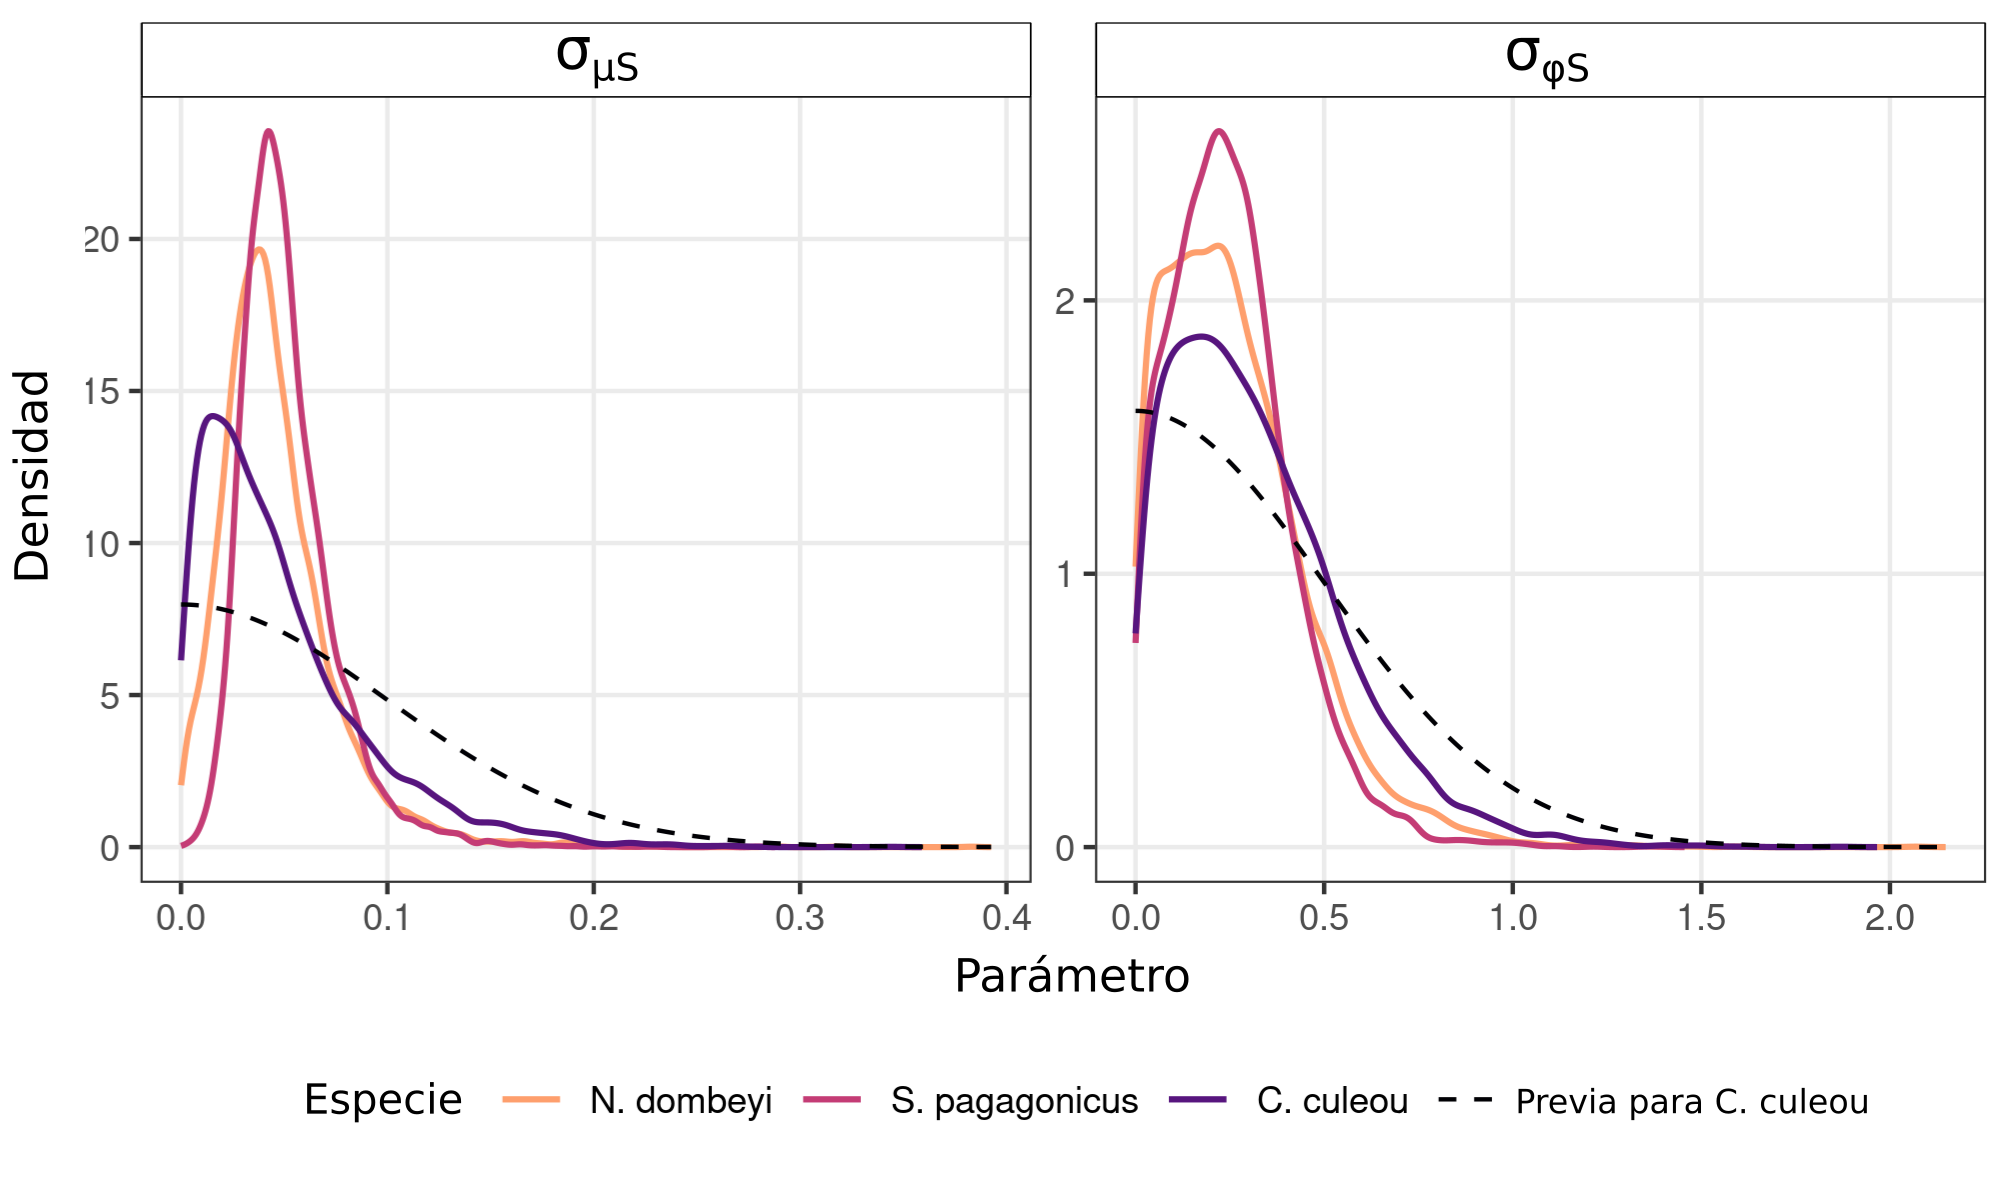
\includegraphics{figuras/cap2/S17) priors.png}
\end{center}
\end{figure}

Para todos los modelos de humedad de combustible, corrimos 10 cadenas durante 1000 iteraciones después de la fase de calentamiento (1500 para la mezcla de combustibles vivos, 2500 para las varillas de combustible de 1 h), y el número de iteraciones de calentamiento por cadena varió según el tipo de combustible: 12000 para \textit{C. culeou}, 1500 para la mezcla de combustibles vivos y 1000 para los demás tipos de combustible. El calentamiento más largo para algunos modelos fue necesario para evitar transiciones divergentes durante la fase de muestreo, y el mayor número de muestras en algunos tipos de combustible fue necesario para alcanzar un tamaño efectivo de muestra alto. A lo largo de todos los modelos de humedad de combustible y parámetros (incluyendo cantidades derivadas calculadas en Stan), el valor máximo de $\hat{\text{R}}$ fue 1.0086, lo que indica convergencia, y el tamaño efectivo de muestra más pequeño fue 826.7.